\documentclass{article}
\usepackage{hyperref}
\usepackage{graphicx}
\usepackage{parskip}  % http://ctan.org/pkg/parskip
\usepackage[T1]{fontenc}
\usepackage{caption}
\usepackage{subcaption}
\usepackage[margin=0.5in]{geometry}

% Make links look pretty in PDFs
\hypersetup{colorlinks=true, urlcolor=blue} 

\begin{document}
\title{HestiaPi Owners Manual}
\author{HestiaPi Community}
\maketitle

\tableofcontents
\newpage

\section{Software}
\subsection{Quick Installation}
To make it easier for new users, HestiaPi offers ready-to-burn image files for your SD card.

If you bought your HestiaPi with an SD card, skip this step.

With the image file downloaded, you need to use an image writing tool (we prefer
Etcher from below links) to install it on your SD card. You can't simply
copy-paste it. If you downloaded a ZIP version, unzip the .img file first before
the next step.

For experienced Linux users, just use dd to write to the block device (SD card)
and use the conv=fsync to make sure everything gets written.  For a more
detailed set of instructions, choose the right guide for your system below
(courtesy of Raspberry Pi website -- thanks):

\begin{itemize}
\item \href{http://www.raspberrypi.org/documentation/installation/installing-images/linux.md}{Linux}
\item \href{http://www.raspberrypi.org/documentation/installation/installing-images/mac.md}{Mac OS}
\item \href{http://www.raspberrypi.org/documentation/installation/installing-images/windows.md}{Windows} (avoid if you can, as people have reported issues flashing their card from Windows)
\end{itemize}



\subsection{Manual Installation}
For people who want to install everything step-by-step, or just see how it is
done, the process is automated in
\url{https://gitlab.hax0rbana.org/public-repos/raspberrypi-automation/}.

That repo is not specific to the HestiaPi, it automates building multiple
Raspberry Pi images that someone might want for their projects. The main file
that is relevant to the HestiaPi project is hestiapi.yml.

The README file in that repo has the latest information on exactly how to build
the image, but the general process to build this at the time of writing is as
follows:

\begin{verbatim}
# Install the necessary software
apt-get update && apt-get install -y ansible xz-utils ansible

# Get a fully patched Raspberry Pi image
PLAYBOOK=upgrade.yml ./build_emulator.sh arm1176 bullseye wrapper_ansible.sh

# Configure that image to be a HestiaPi
PLAYBOOK=hestiapi.yml EXTRA_VARS="hestiapi_version=v1.4-dev" \
        ./build\_emulator.sh arm1176 bullseye wrapper_ansible.sh

# At this point you will have your HestiaPi image at the following location
ls -l qemu-rpi/2022-09-22-raspios-bullseye-armhf-lite.img
\end{verbatim}

These instructions were tested on Ubuntu and should work on any Debian-based
Linux distribution.


\subsection{Software Architecture} \label{Software Architecture}
\input{software_architecture}


\section{Hardware}
\subsection{Bill of Materials (BOM)}
This is the bill of materials to make your own HestiaPi.  The AC/DC converter
allows your HestiPi to be powered by the HVAC unit, but it requires that your
HVAC system has a common wire.  If your system does not have a common wire
(e.g., if it only has Red, Green, White, and Yellow wires), the AC/DC converter
will not work.  In that case, you will need a 5V/1A DC power supply, and your
hestia will need to be plugged into a wall outlet.

The LCD headers need to be 15mm long, with 12mm of that being on the top of the
board.  Standard headers are not long enough to allow the LCD to clear the
relays.

\begin{enumerate}
  \item Printed Circuit Board -- Send the 
        \href{https://github.com/HestiaPi/hestia-touch-pcb-dev/tree/master/HestiaPi-ONE/Gerber}{Gerber Files}
        to a shop like \href{https://jlcpcb.com/}{JLCPCB} (or use them to etch
        your own board)
  \item Raspberry Pi Zero W \href{https://www.adafruit.com/product/3400}{AdaFruit} \href{https://smile.amazon.com/Raspberry-Pi-Zero-Wireless-model/dp/B06XFZC3BX/}{Amazon}
  \item 3.5 inch touch screen for Raspberry Pi \href{https://smile.amazon.com/gp/product/B01CNJVG8K/}{Amazon}
  \item 4 relays capabile of handling 24V / 2A -- G3MC-202P-DC5 \href{https://www.mouser.com/ProductDetail/653-G3MC-202P-DC5}{Mouser}
  \item At least 40 standard male 0.1" headers -- \href{https://www.adafruit.com/product/3009}{AdaFruit}
  \item Reset switch -- TL1105WF160Q \href{https://www.mouser.com/ProductDetail/612-TL1105W}{Mouser}
  \item A six-post terminal block -- TB003-500-P06BE \href{https://www.mouser.com/ProductDetail/490-TB003-500-P06BE}{Mouser}
  \item BME280 sensor -- SEN0372 \href{https://www.mouser.com/ProductDetail/426-SEN0372}{Mouser}
  \item Cable for BME280 sensor \href{https://smile.amazon.com/dp/B0789F523N/}{Amazon}
  \item LCD headers, 2x13 extra long headers (total length should be 15mm, 12mm from board to tip) \href{https://www.adafruit.com/product/400}{AdaFruit} (requires adjusting pins)
  \item AC/DC converter -- \href{https://smile.amazon.com/dp/B00RE6QN4U/}{Amazon}
\end{enumerate}


\subsection{PCB Soldering}
\subsubsection{Instructions}
This guide describes the steps required to solder and assemble HestiaPi Touch ONE
from parts.  Assembly with the case and wall is covered in Section
\ref{Wall Installation ONE}.

\begin{enumerate}
  \item Solder standard headers onto PCB for the pi (figure \ref{fig:pi_headers})
	  Make sure you don't miss the reset pin at the right, just below the
		block of 2x20 pins
  \item Solder the pi onto those headers (figure \ref{fig:pi})
  \item Put terminal block and sendor headers in place and solder them on (figures
	  \ref{fig:terminal_block_in_place} and \ref{fig:terminal_block_soldered})
  \item Solder relays in place (figure \ref{fig:relays})
  \item Solder the headers onto the BME board (figures \ref{fig:BME} and
	  \ref{fig:BME_soldered})
  \item Solder switch in place (figure \ref{fig:switch})
  \item Pull the long headers so the top of the pin is 12mm off of the board,
	  do this for all of the pins in the LCD headers
	  (figures \ref{fig:header} and \ref{fig:headers})
  \item Solder the LCD headers into place and connect the BME280 board
	  (\ref{fig:fully_assembled})
  \item If using the AC/DC converter, solder that on
\end{enumerate}

\begin{figure}
  \centering
  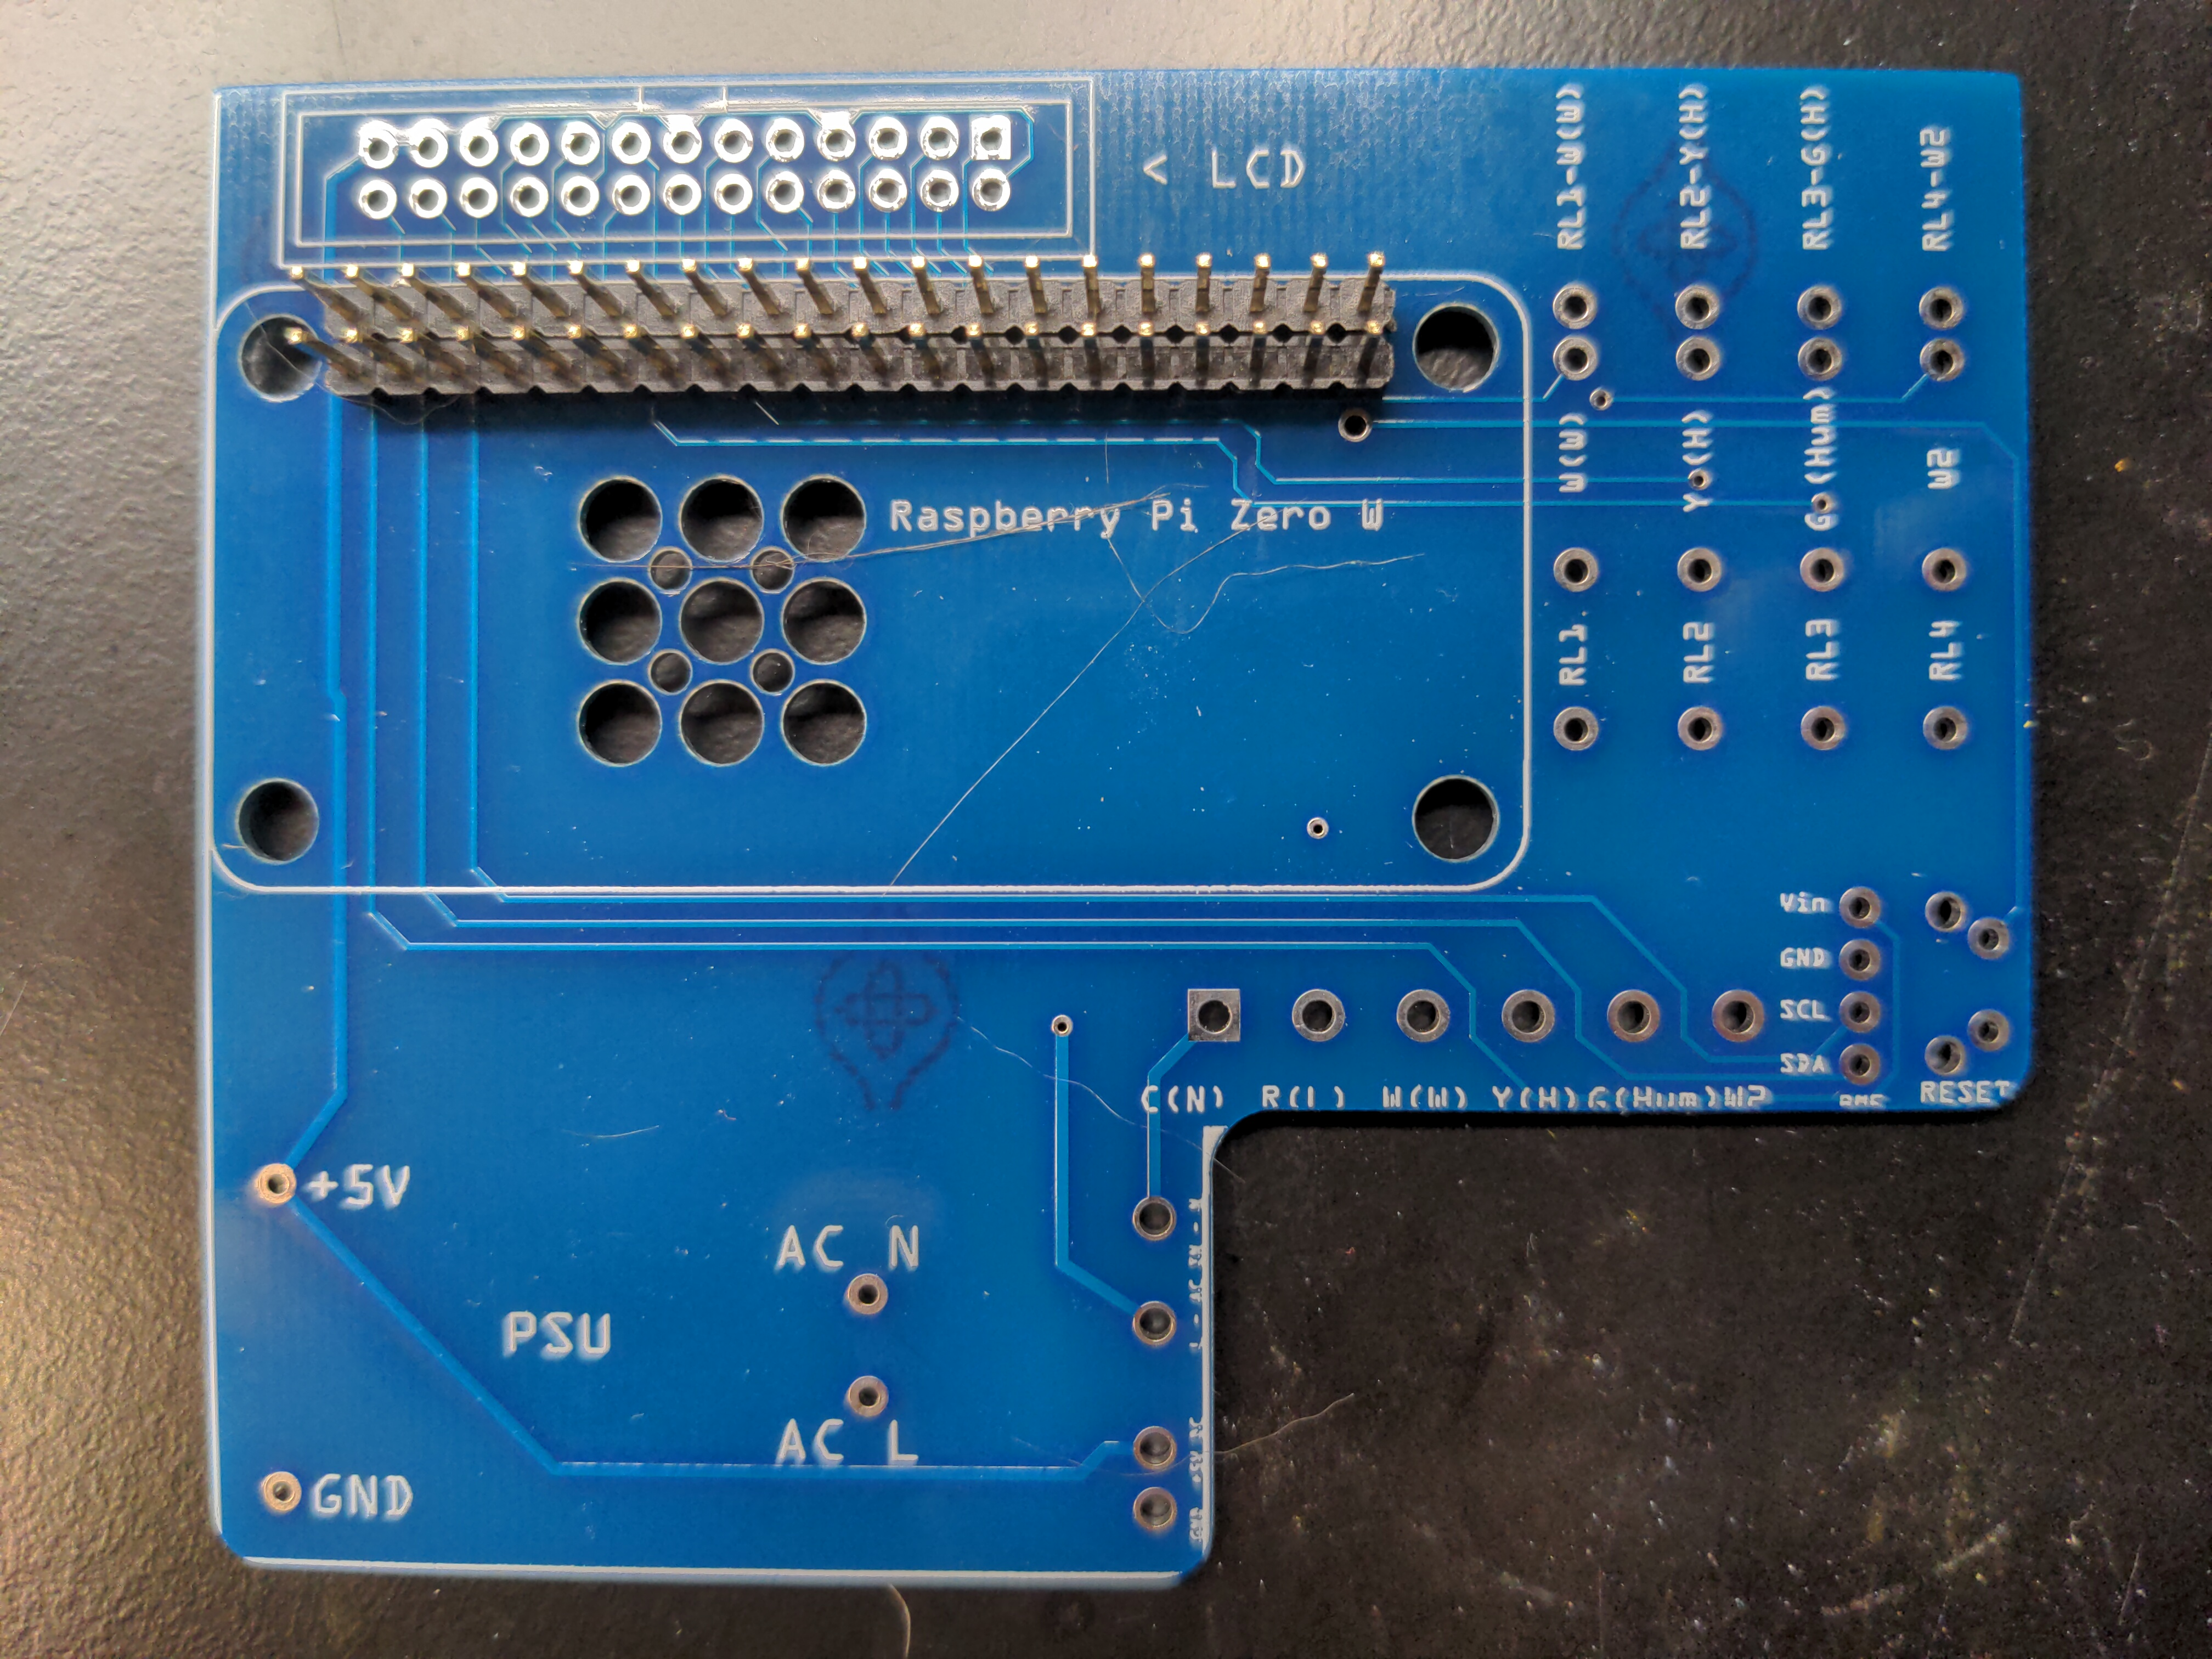
\includegraphics[width=3in]{img/pi_header_placement_soldered_on.jpg}
  \caption{Headers for the pi, don't forget the reset pin like I did here!}
  \label{fig:pi_headers}
\end{figure}
\begin{figure}
  \centering
  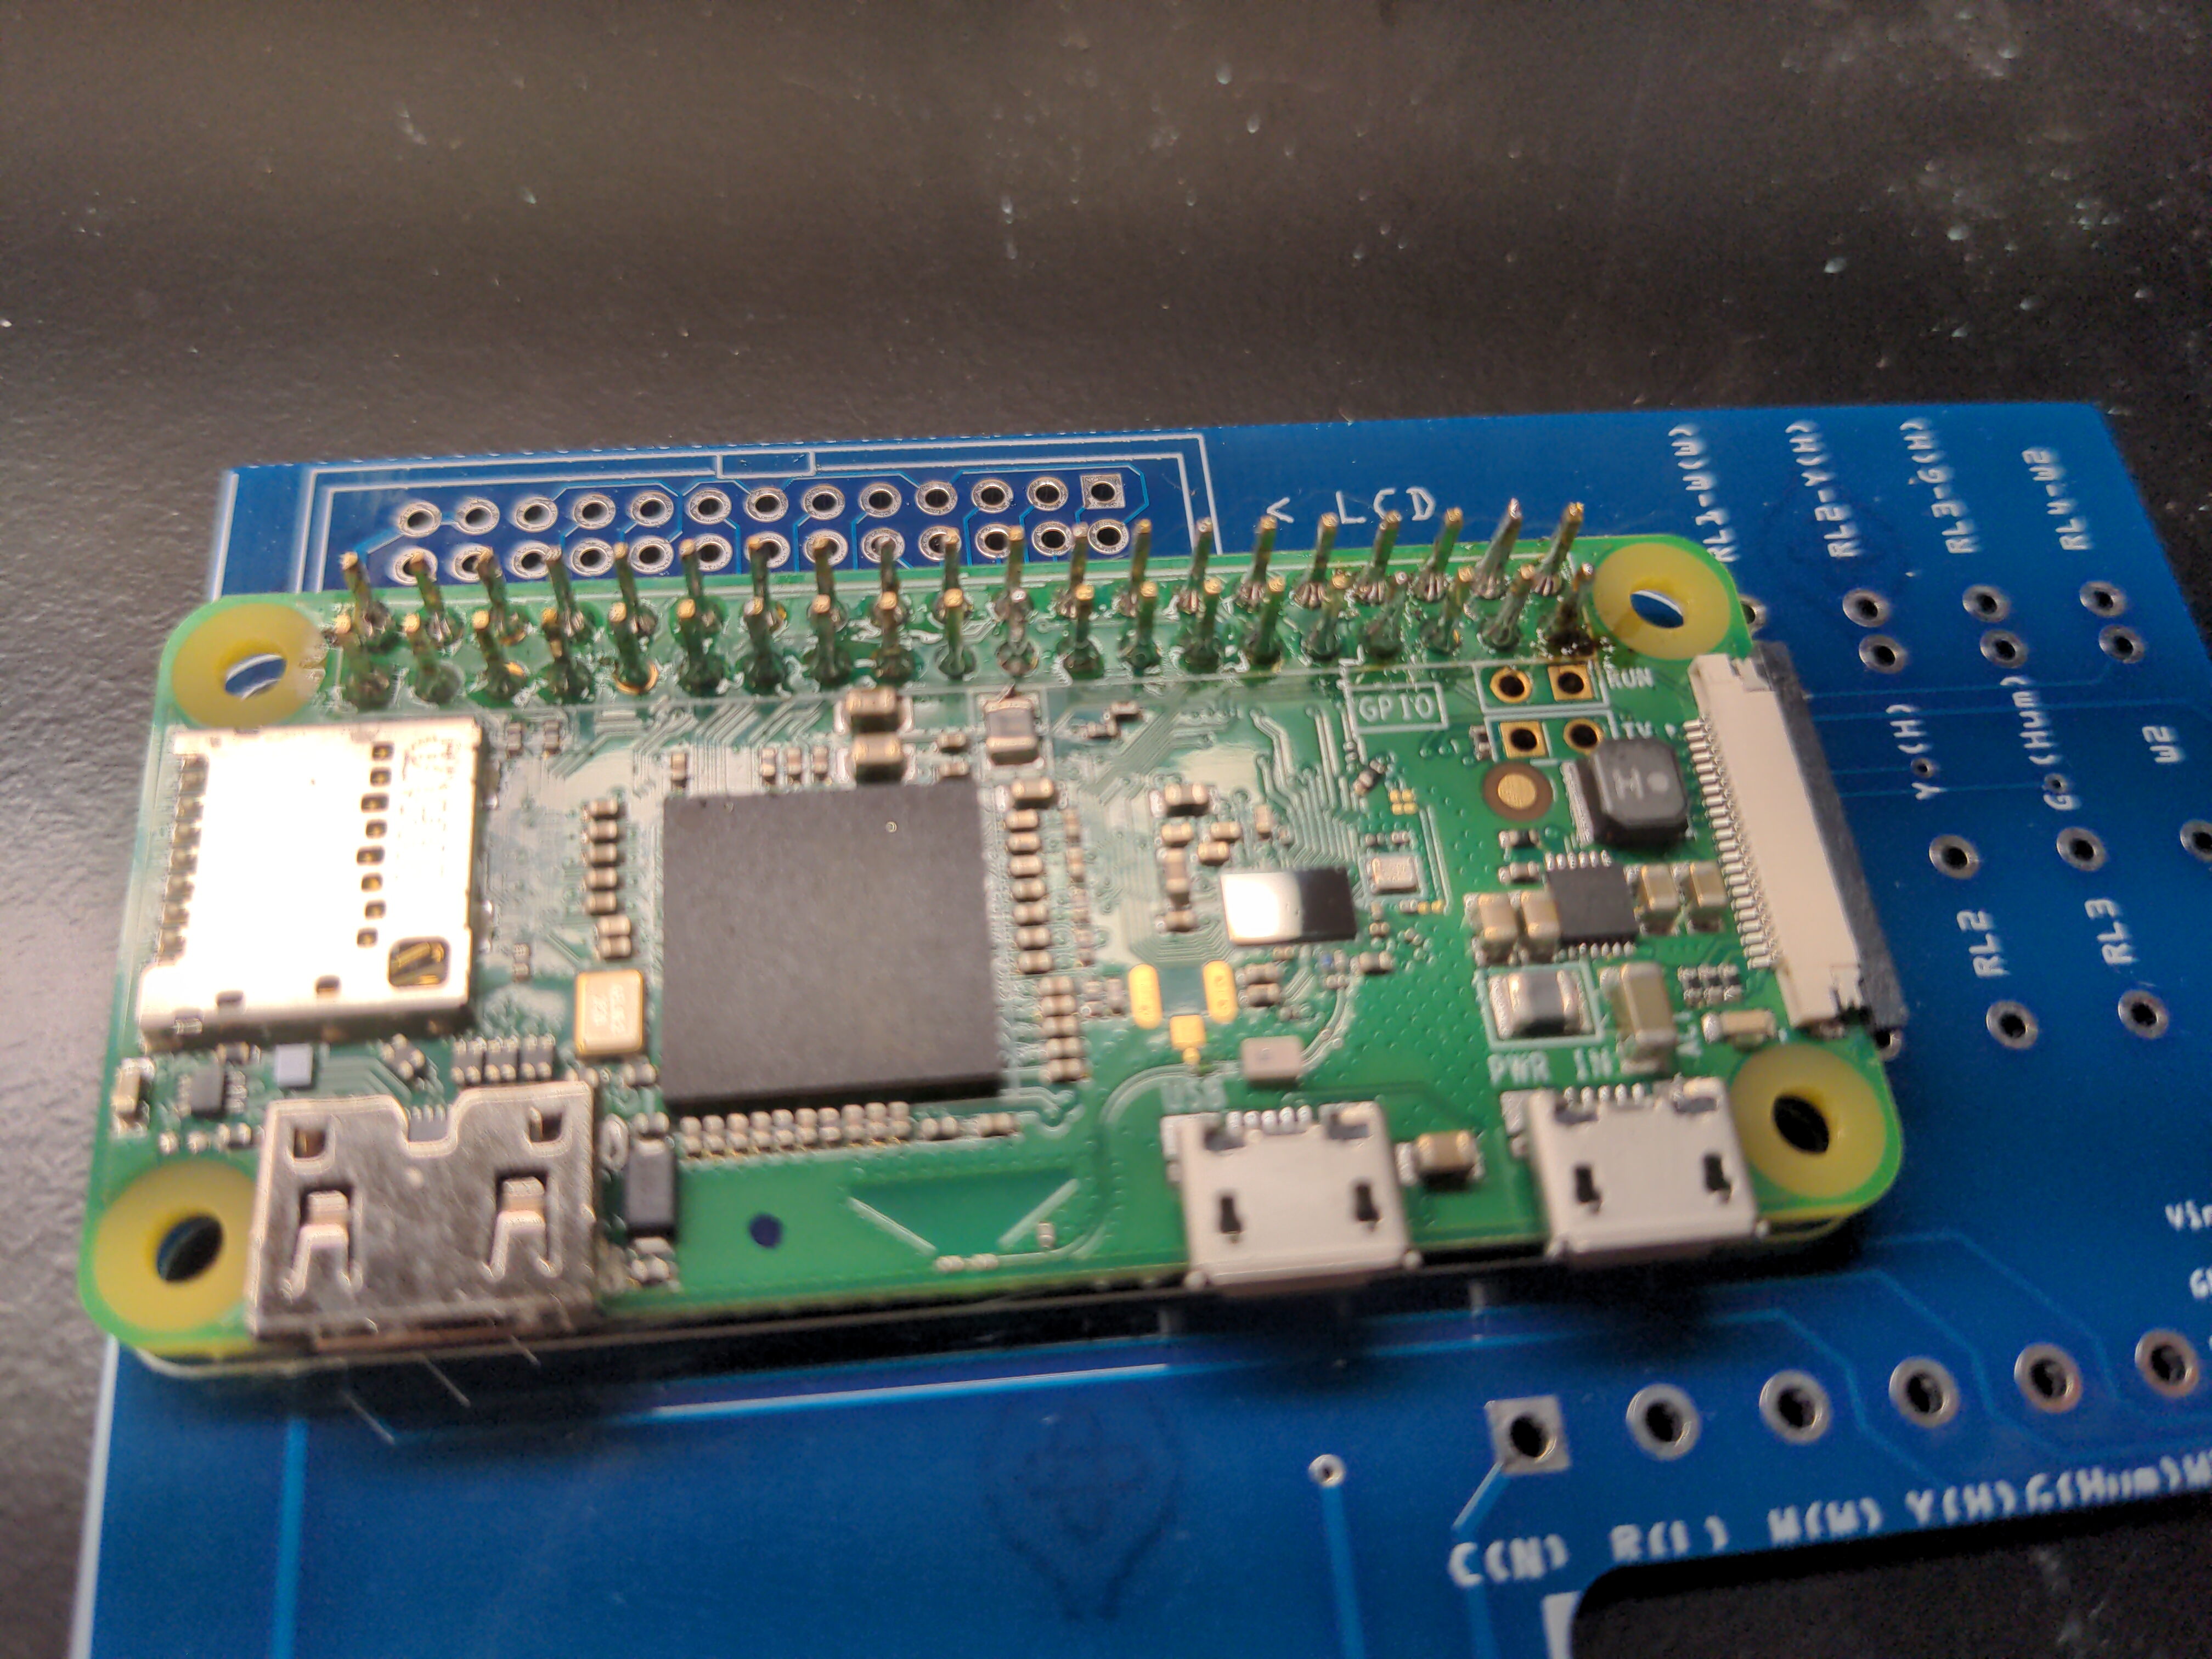
\includegraphics[width=3in]{img/pi_soldered_on.jpg}
  \caption{Pi soldered on, sans the reset pin that I had to go back and patch
	up later}
  \label{fig:pi}
\end{figure}
\begin{figure}
  \centering
  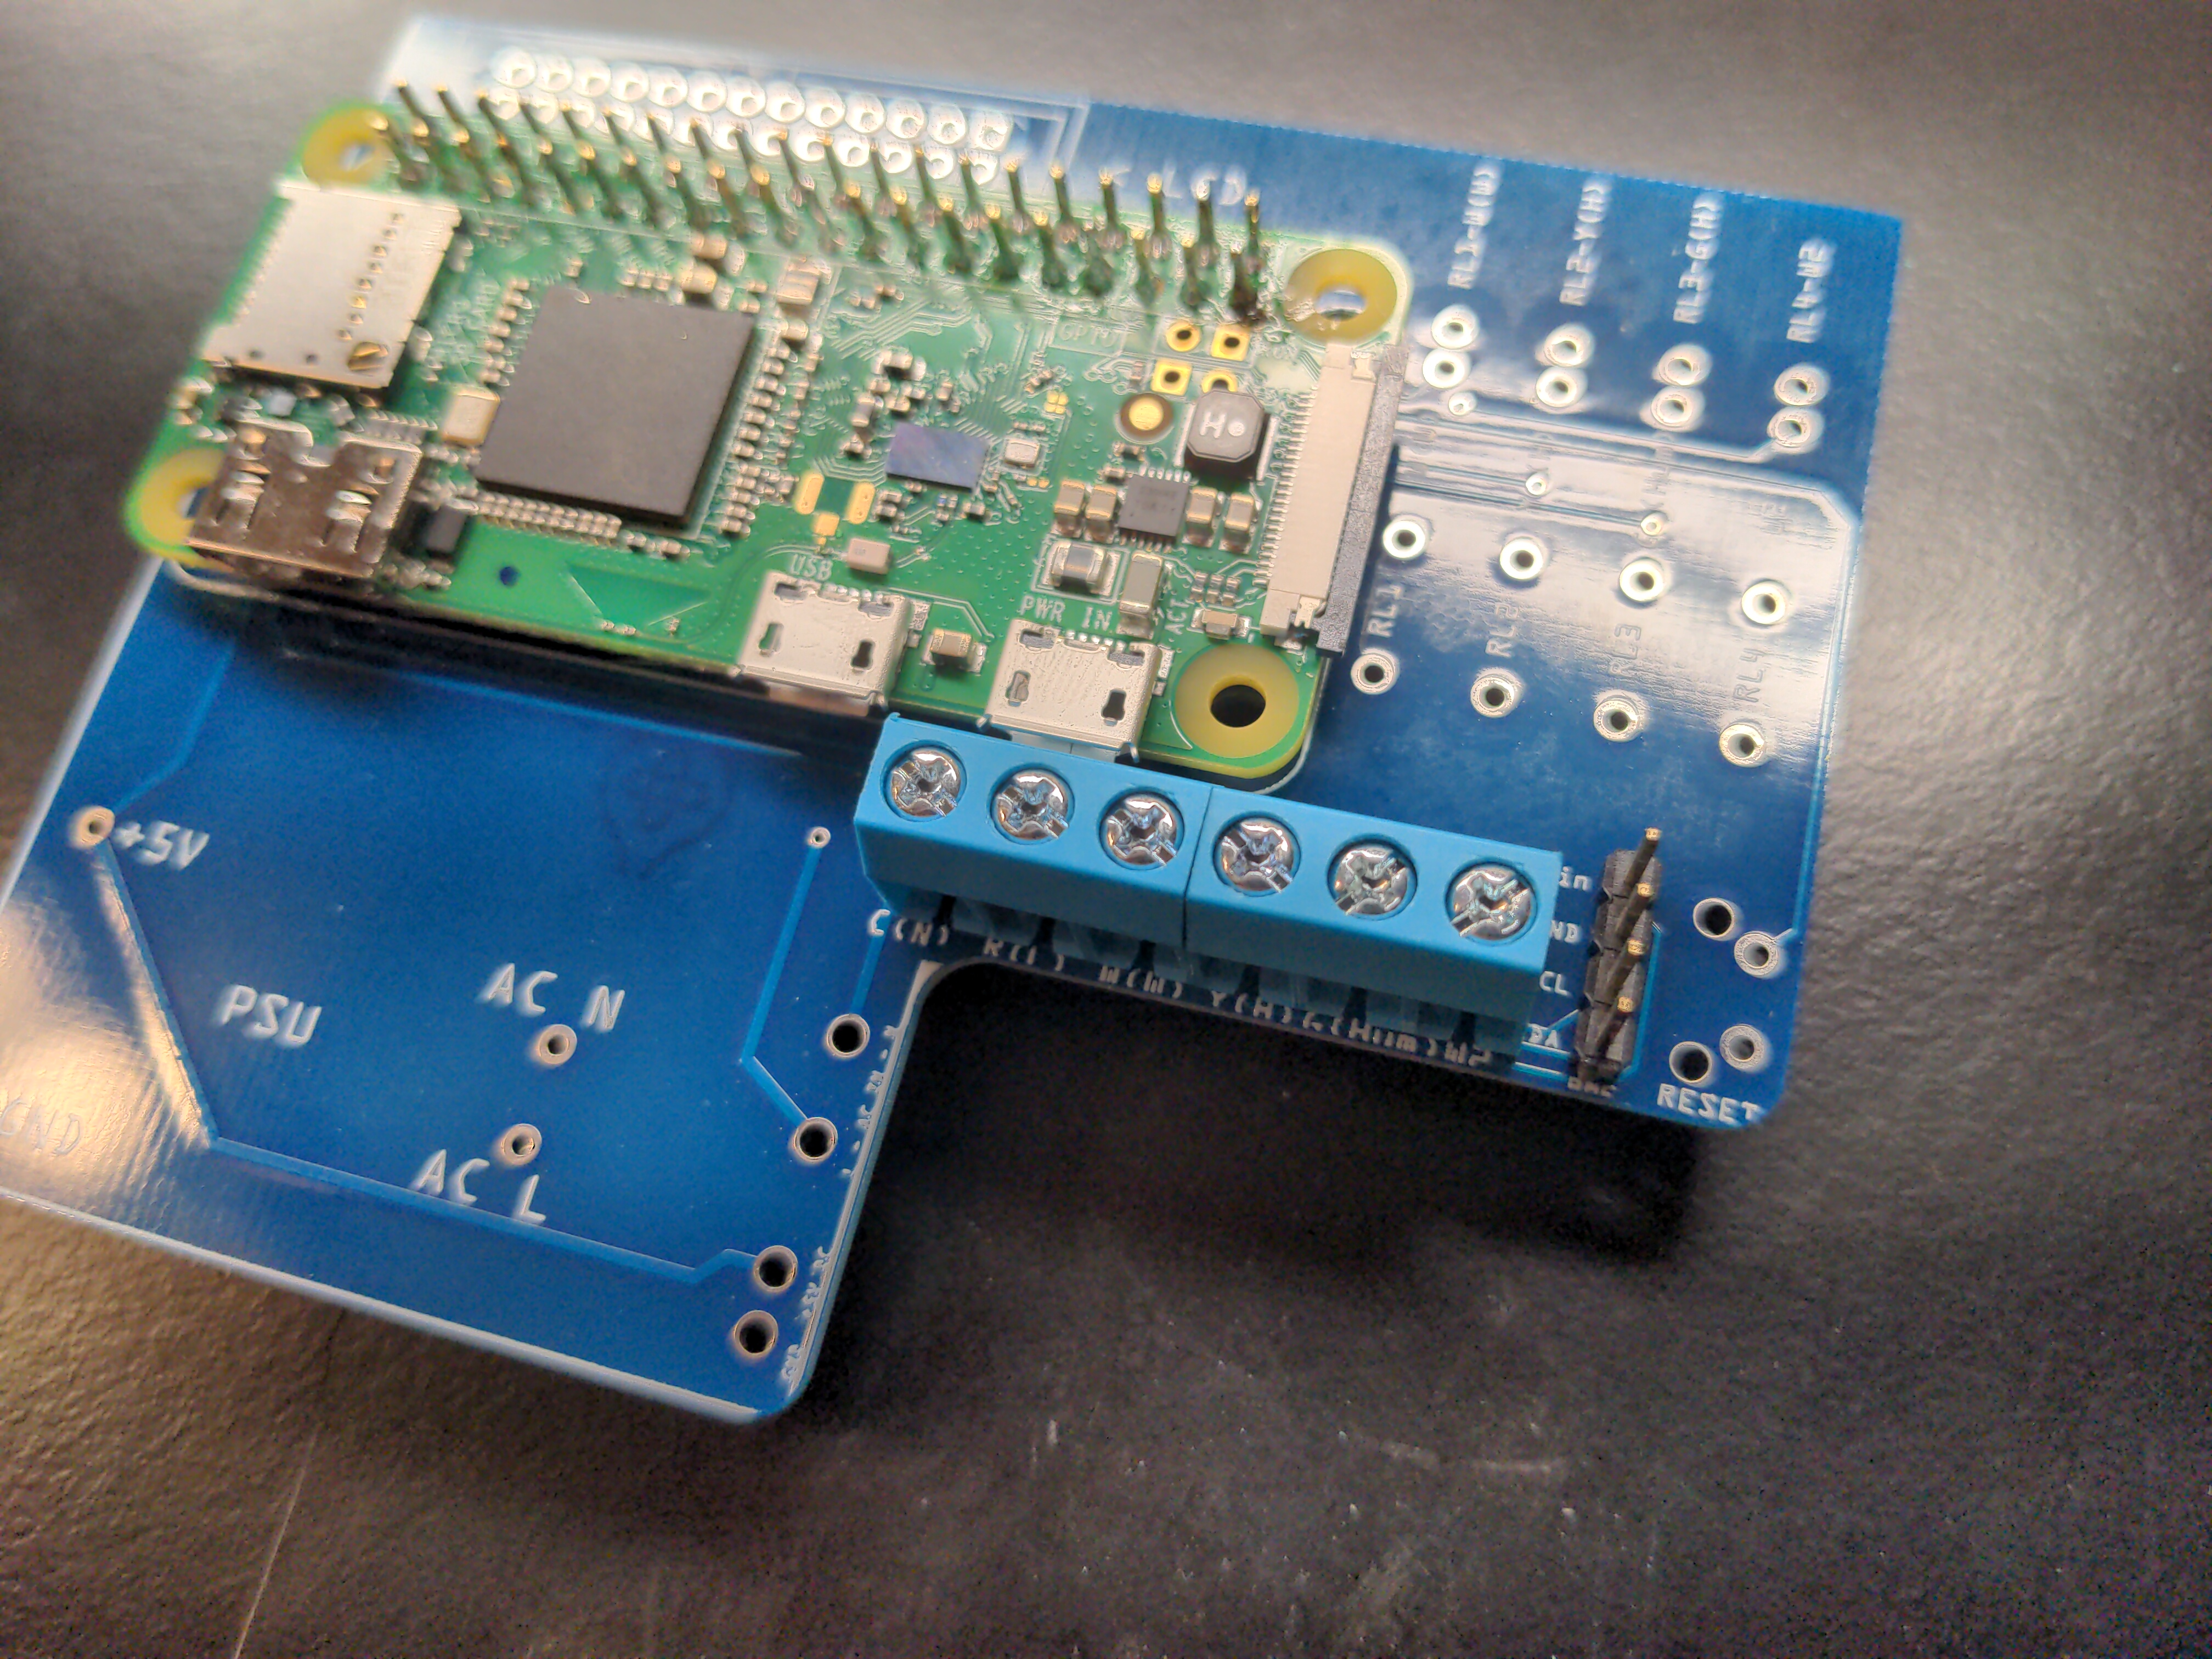
\includegraphics[width=3in]{img/terminal_block_placement.jpg}
  \caption{Terminal block and sensor headers in place}
  \label{fig:terminal_block_in_place}
\end{figure}
\begin{figure}
  \centering
  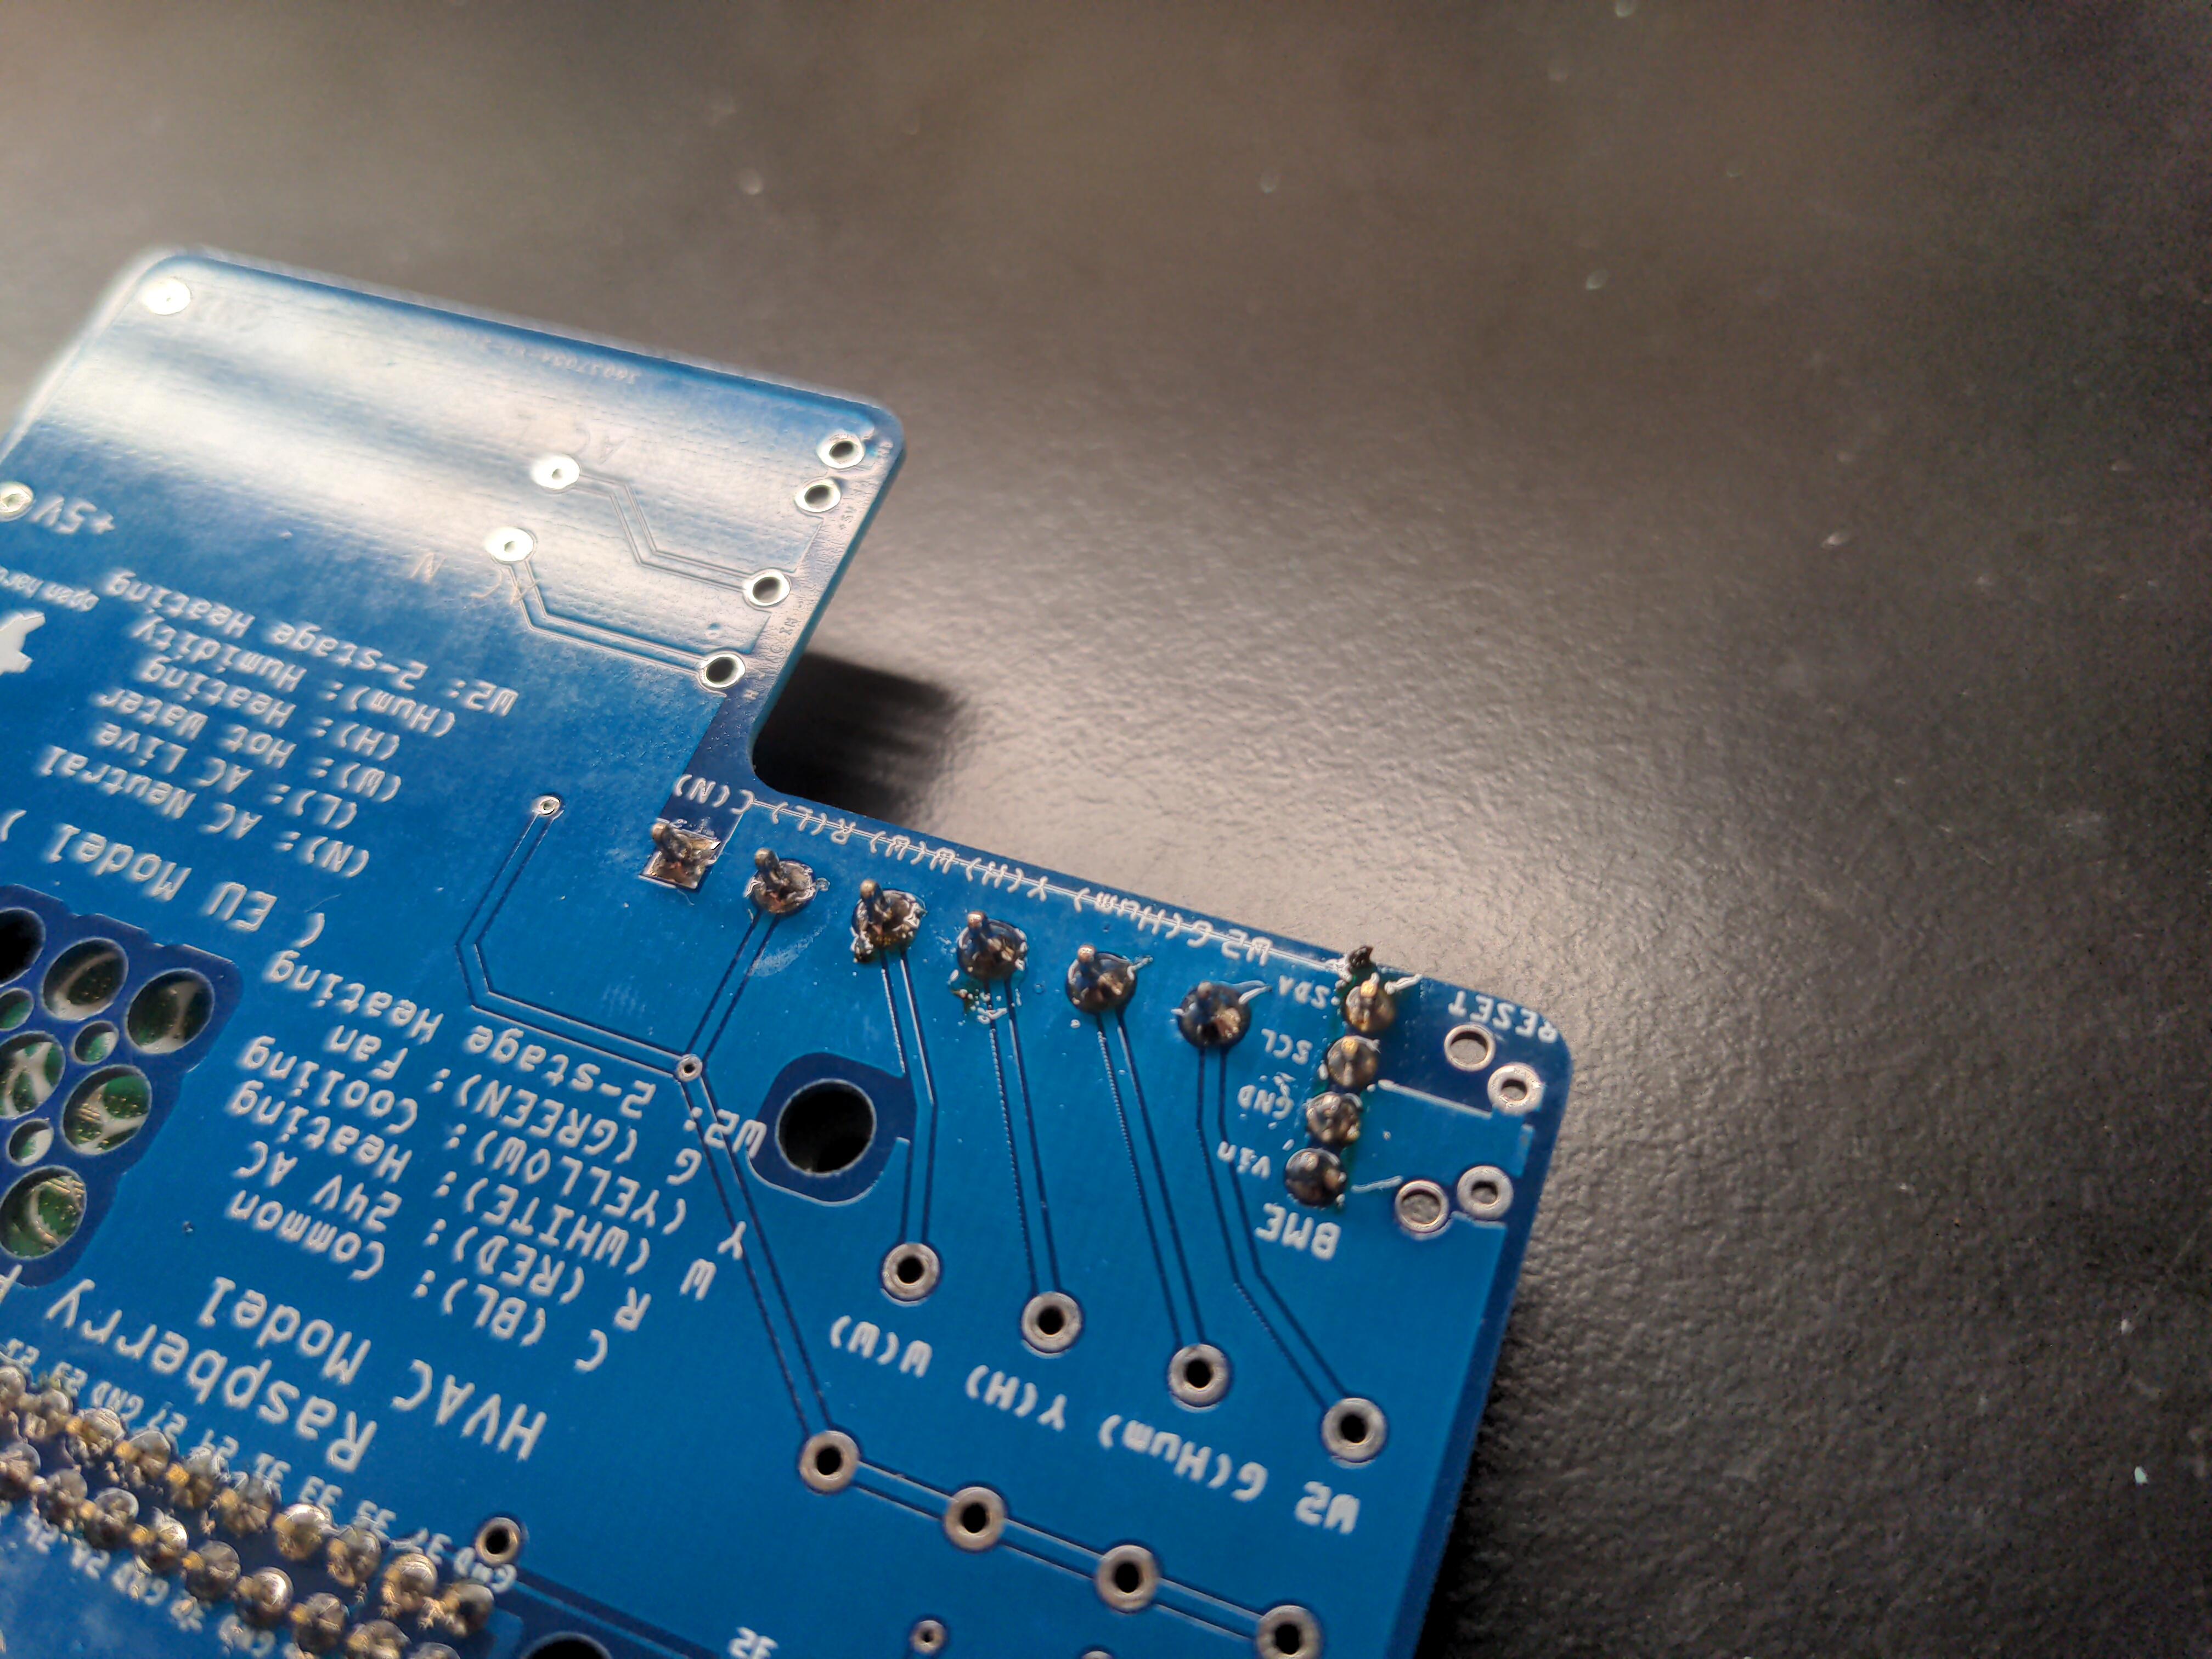
\includegraphics[width=3in]{img/terminal_block_soldered.jpg}
  \caption{Terminal block and sensor headers soldered on}
  \label{fig:terminal_block_soldered}
\end{figure}
\begin{figure}
  \centering
  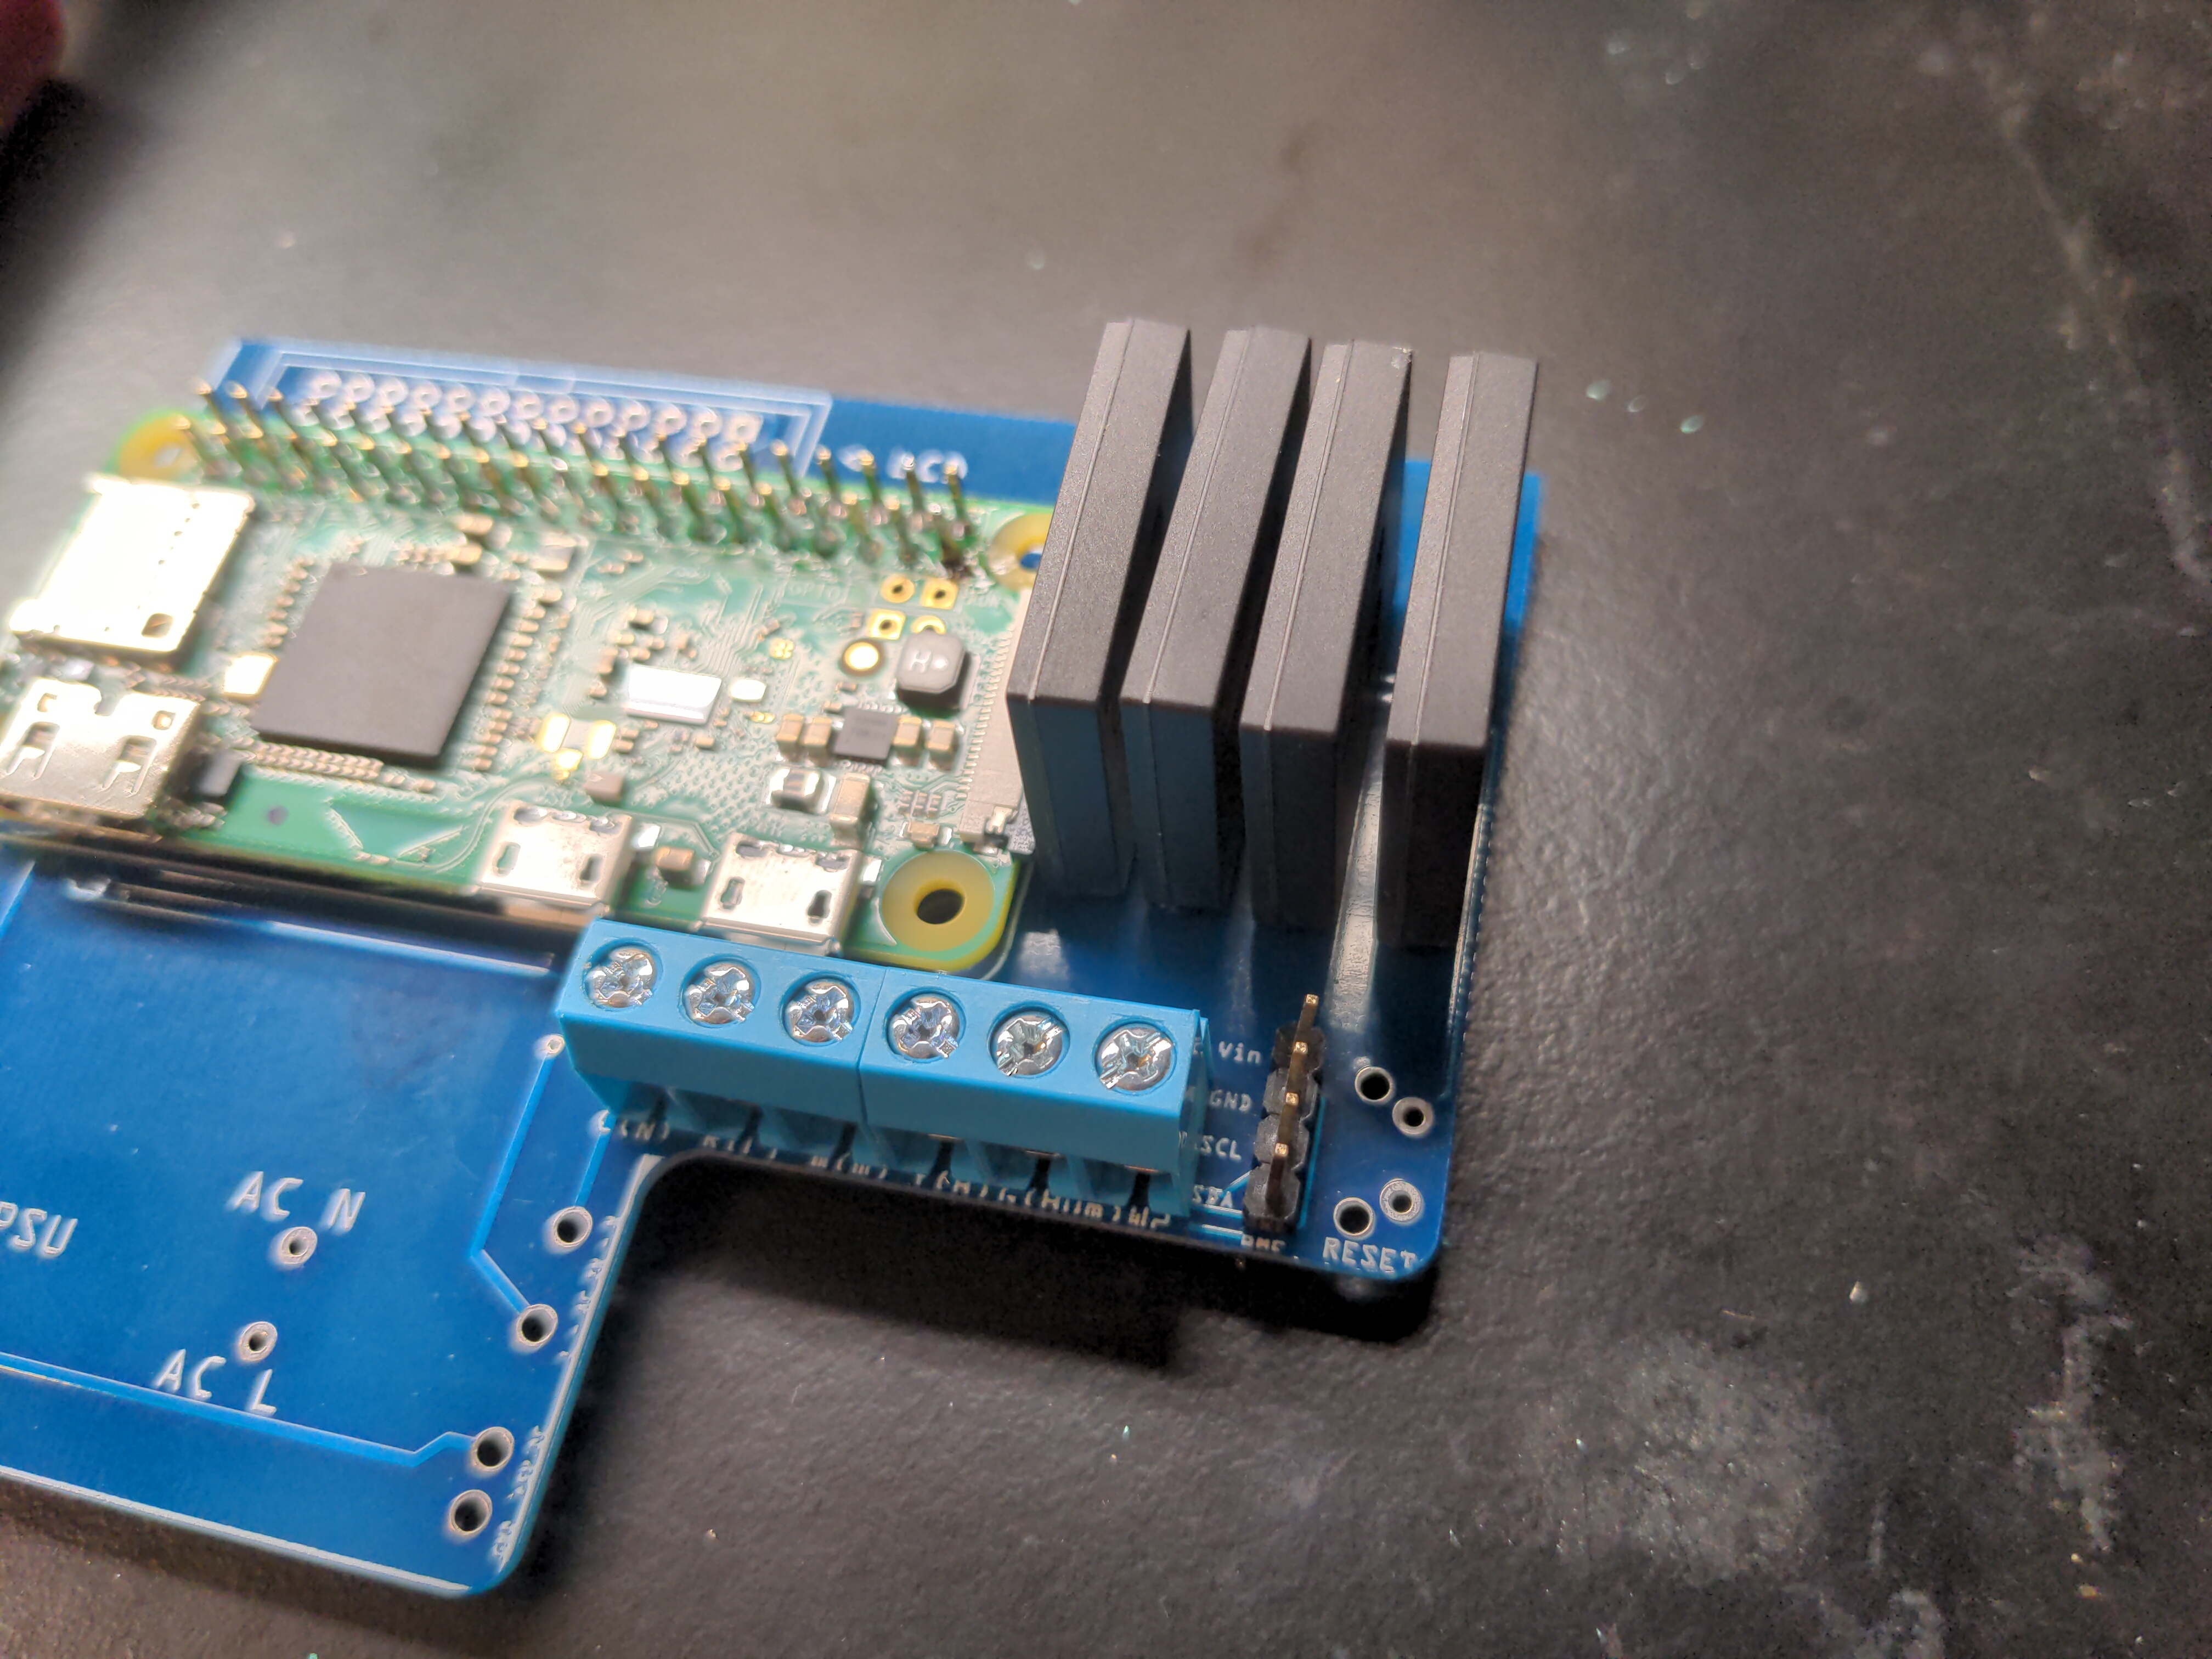
\includegraphics[width=3in]{img/relay_placement.jpg}
  \caption{Relays soldered into place}
  \label{fig:relays}
\end{figure}
\begin{figure}
  \centering
  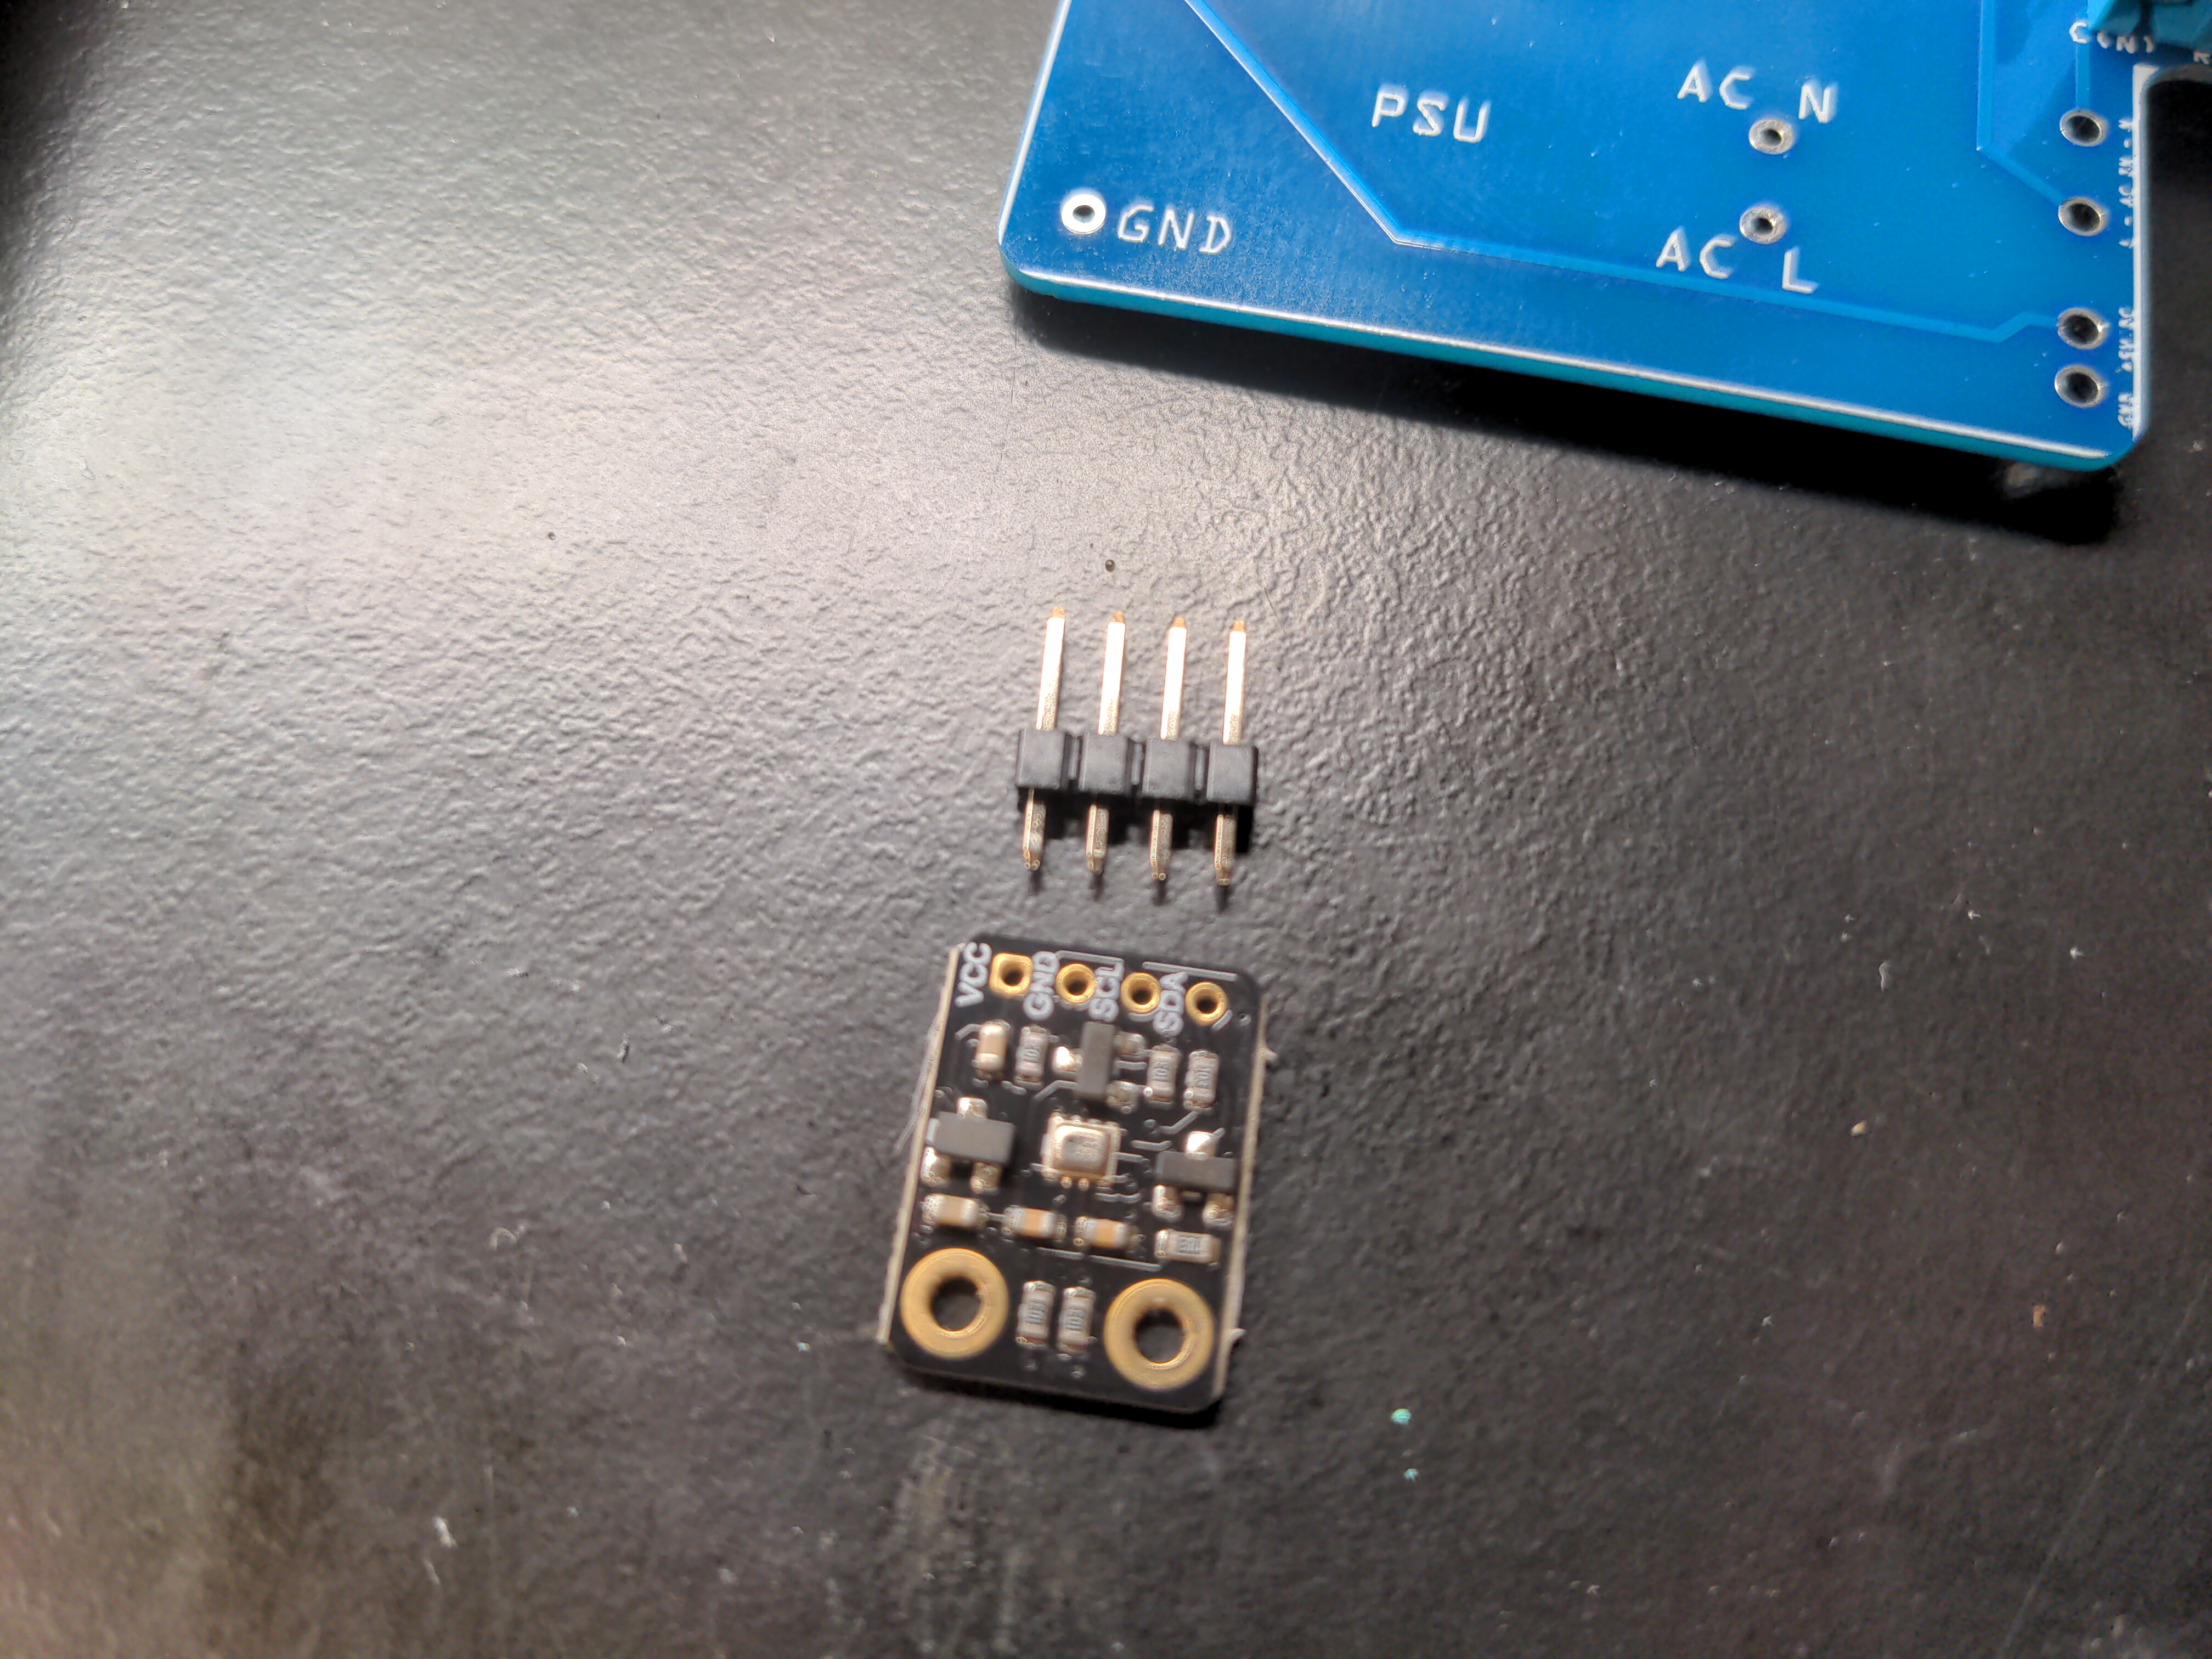
\includegraphics[width=3in]{img/BME280.jpg}
  \caption{BME needs to have headers attached}
  \label{fig:BME}
\end{figure}
\begin{figure}
  \centering
  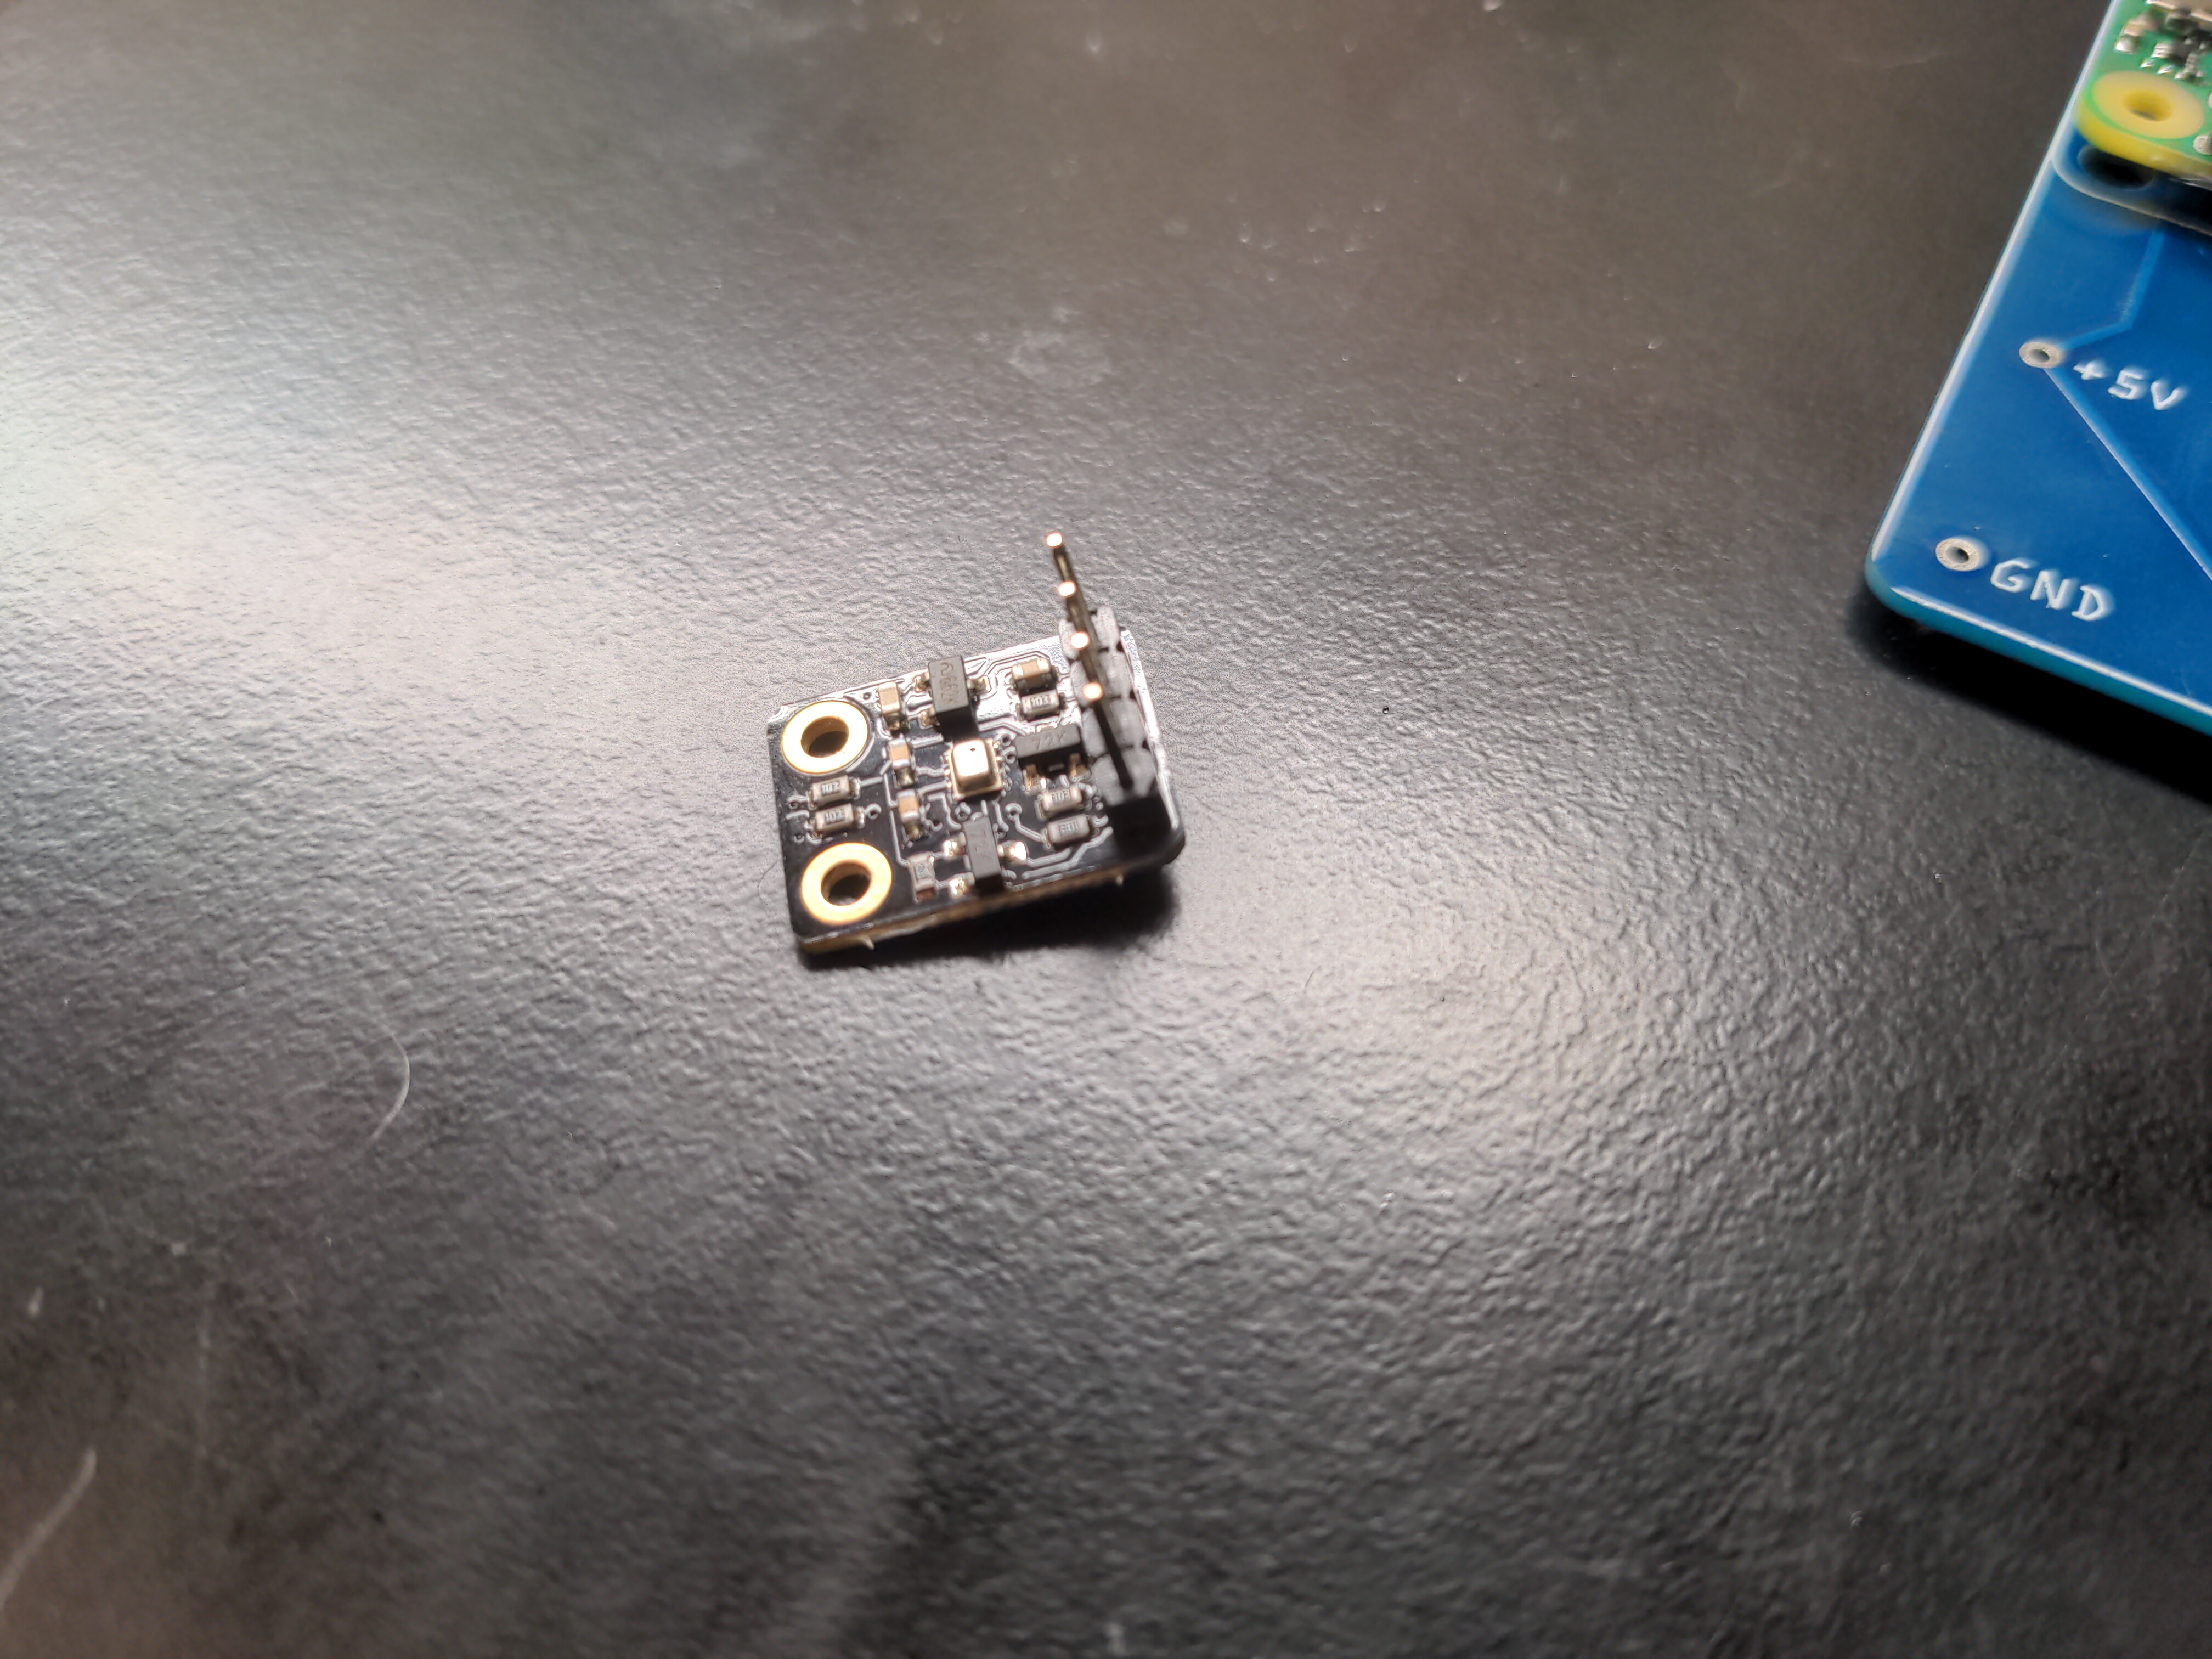
\includegraphics[width=3in]{img/BME280_assembled.jpg}
  \caption{BME with headers soldered on}
  \label{fig:BME_soldered}
\end{figure}
\begin{figure}
  \centering
  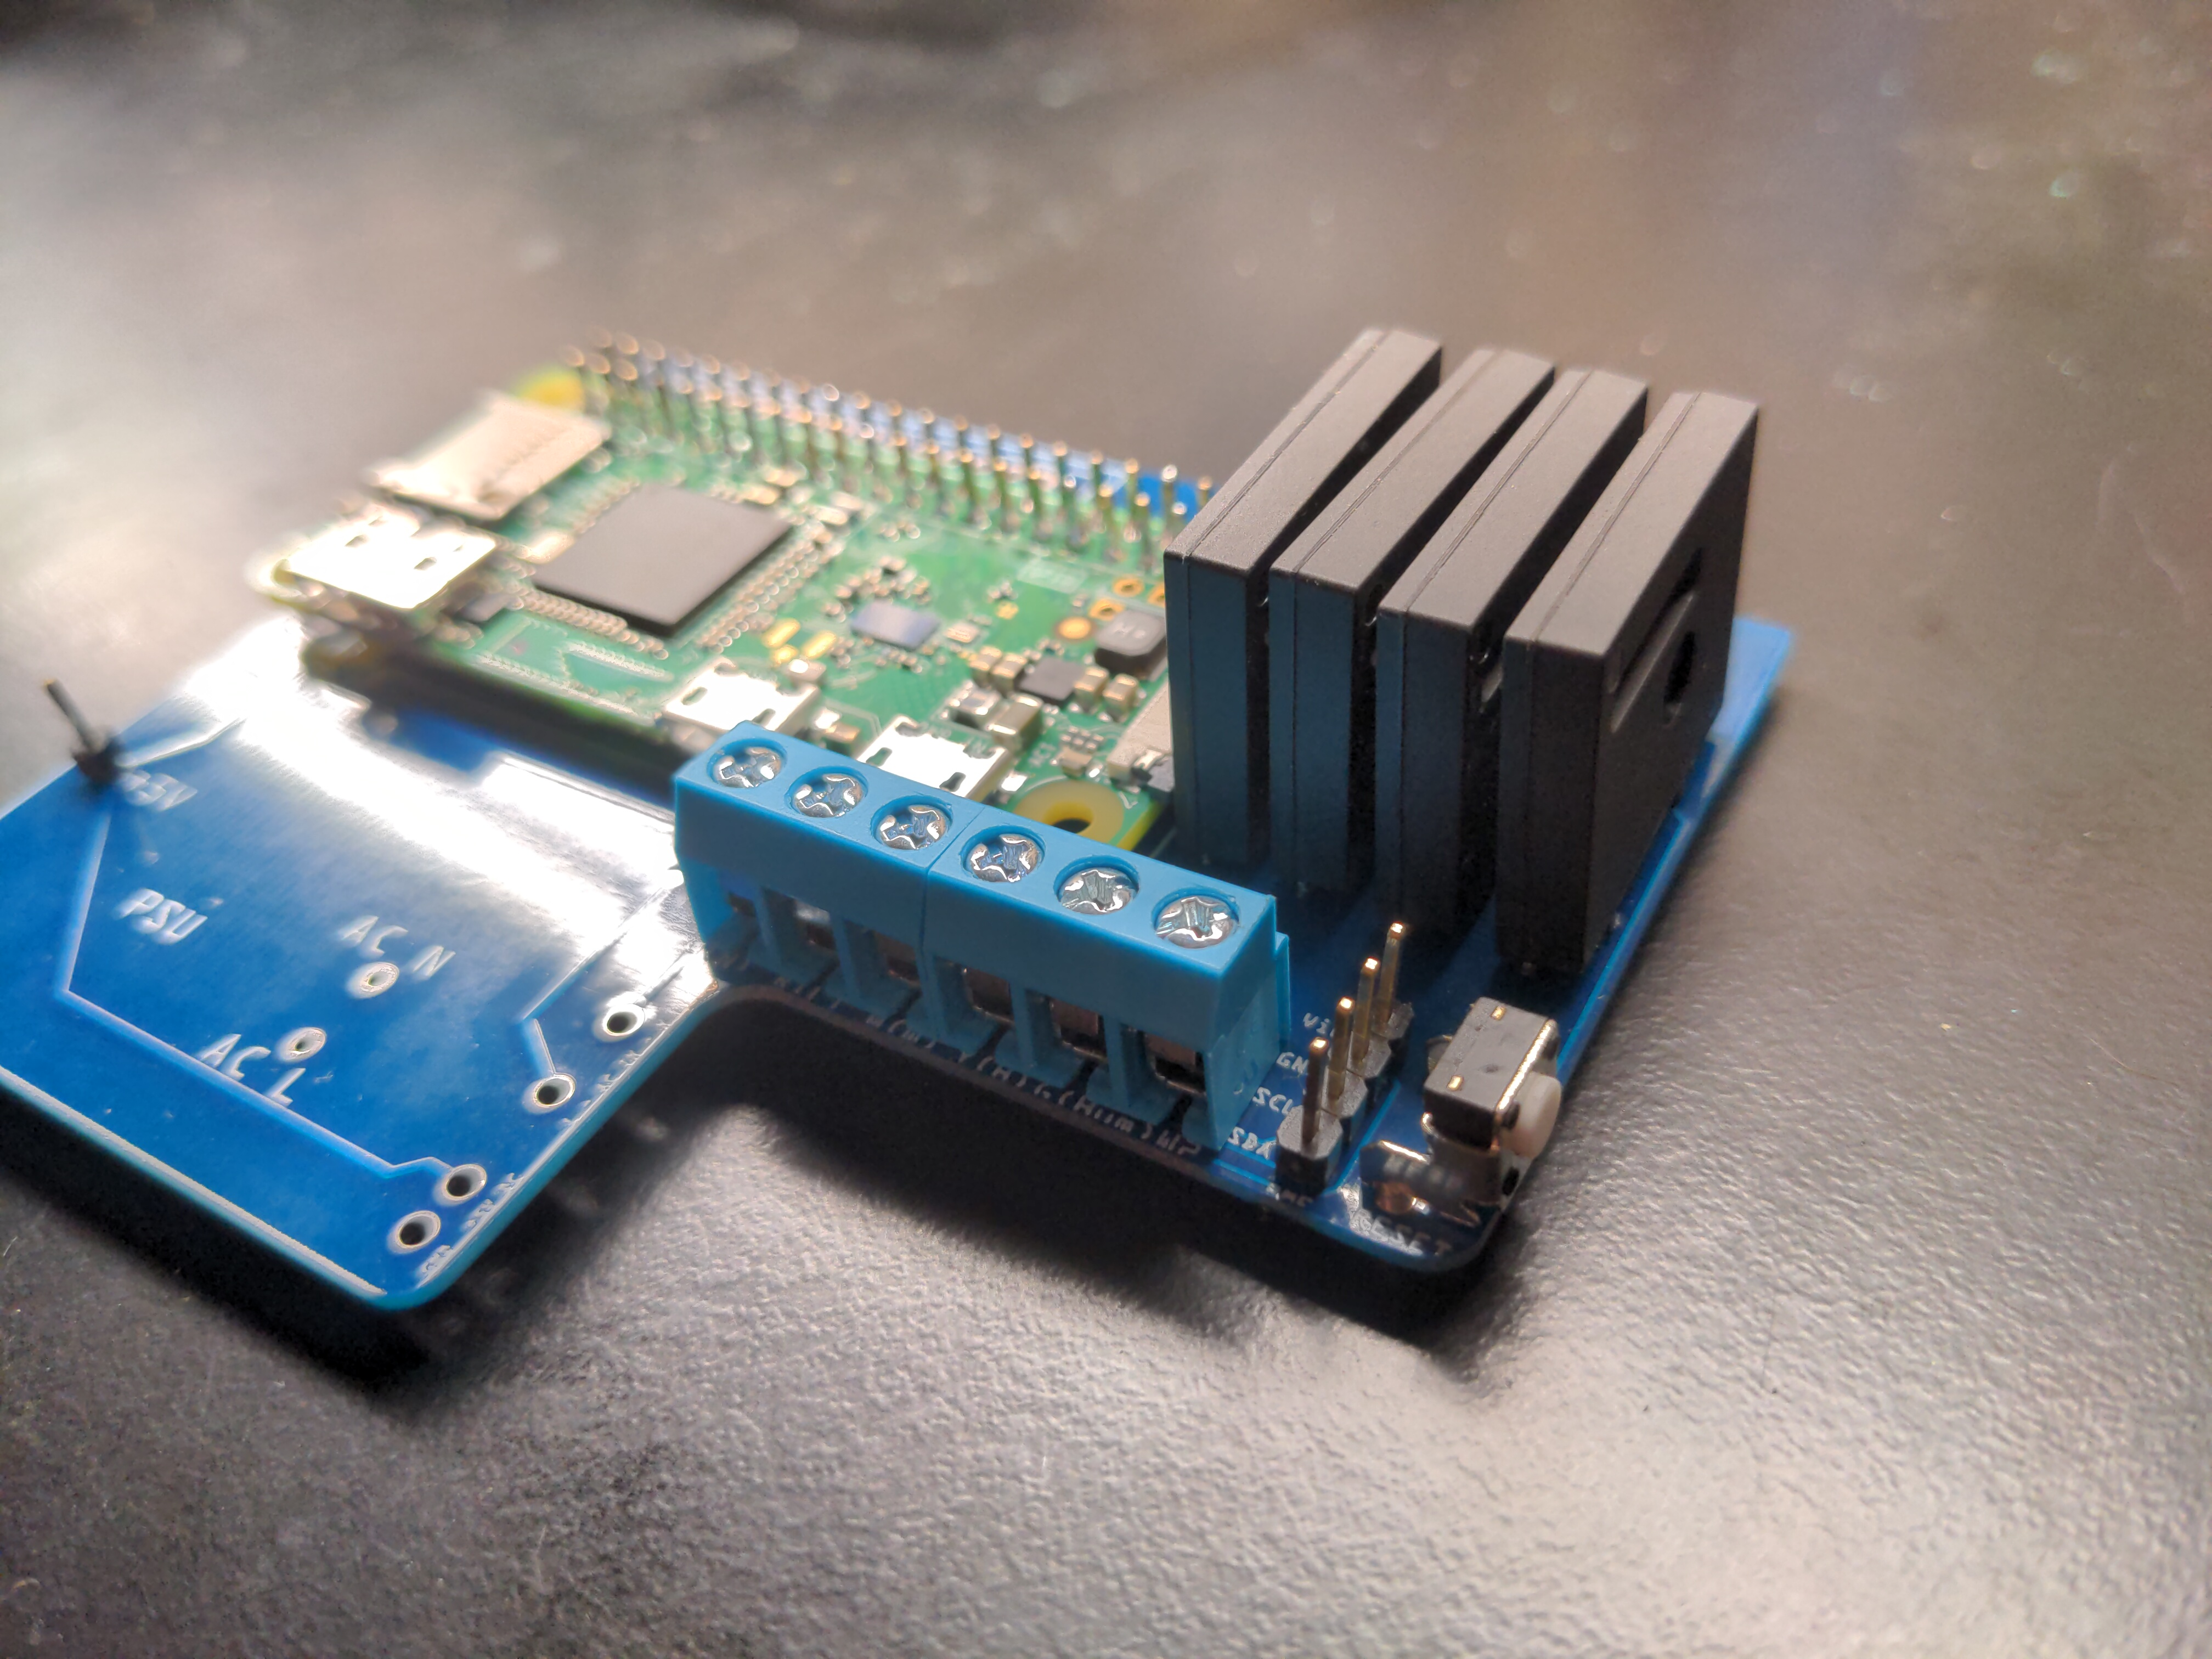
\includegraphics[width=3in]{img/switch.jpg}
  \caption{Solder switch into place}
  \label{fig:switch}
\end{figure}
\begin{figure}
  \centering
  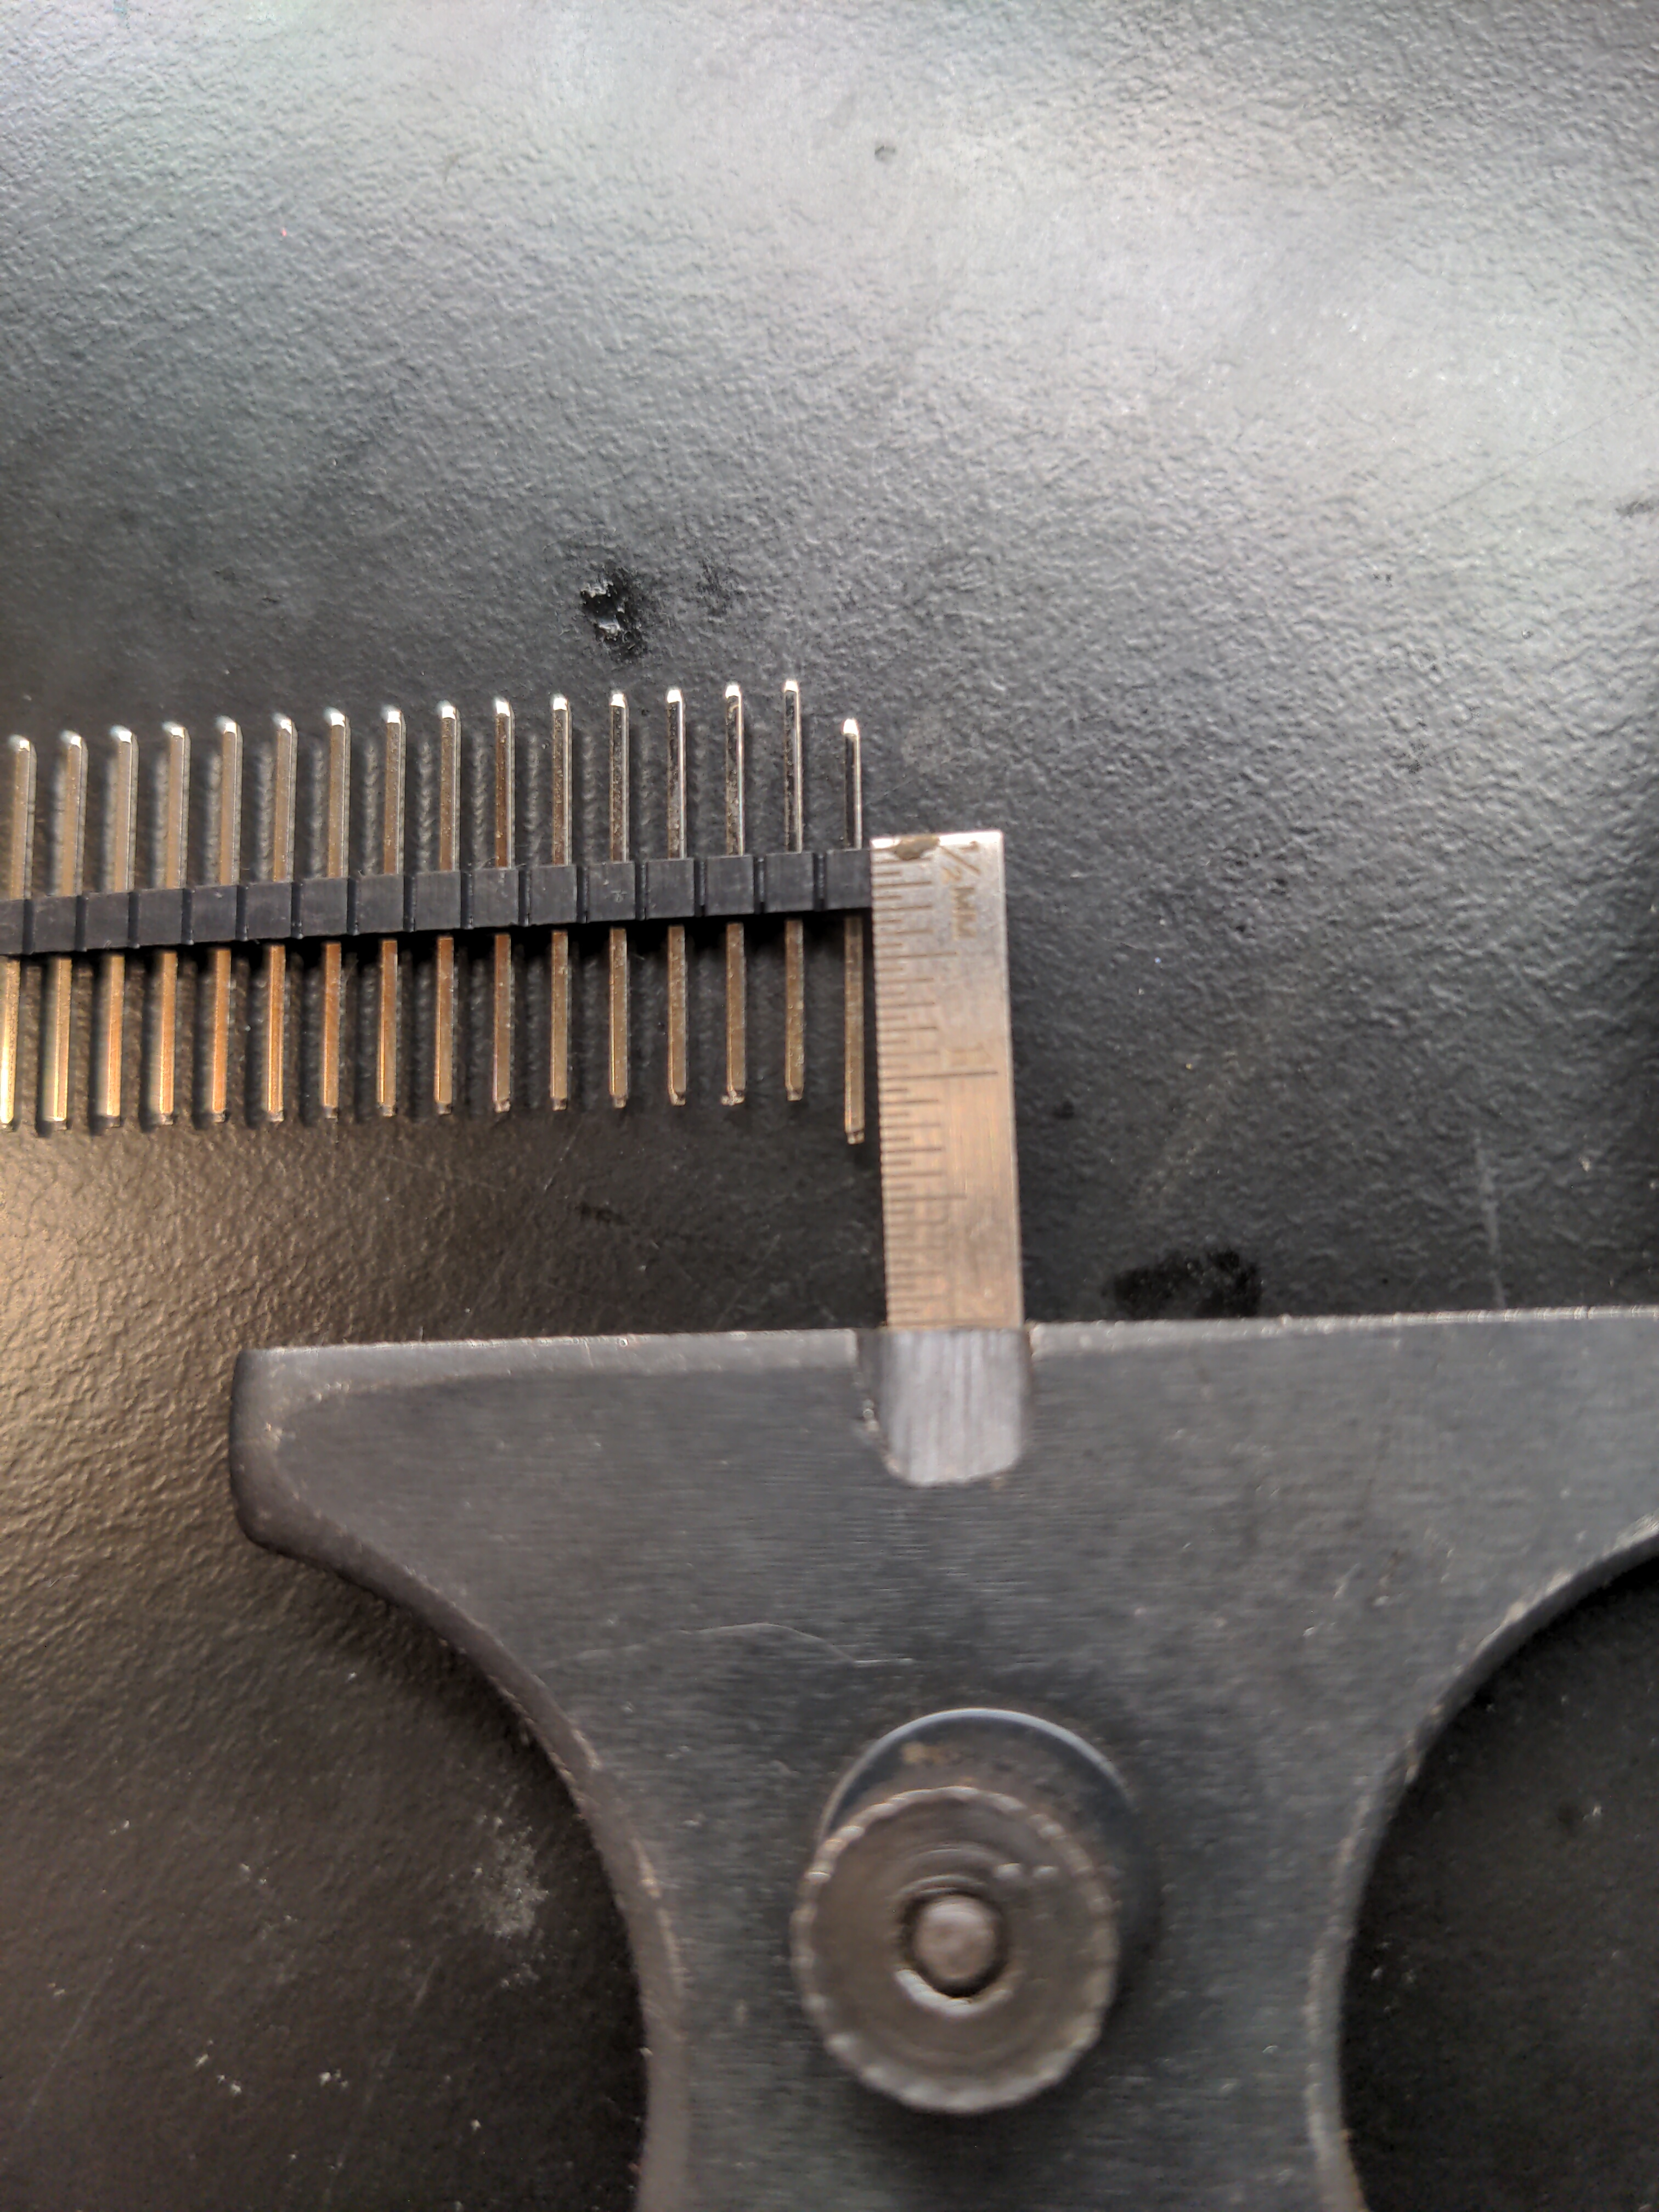
\includegraphics[width=3in]{img/modified_header.jpg}
  \caption{Pin placement adjusted to have 12mm above the board}
  \label{fig:header}
\end{figure}
\begin{figure}
  \centering
  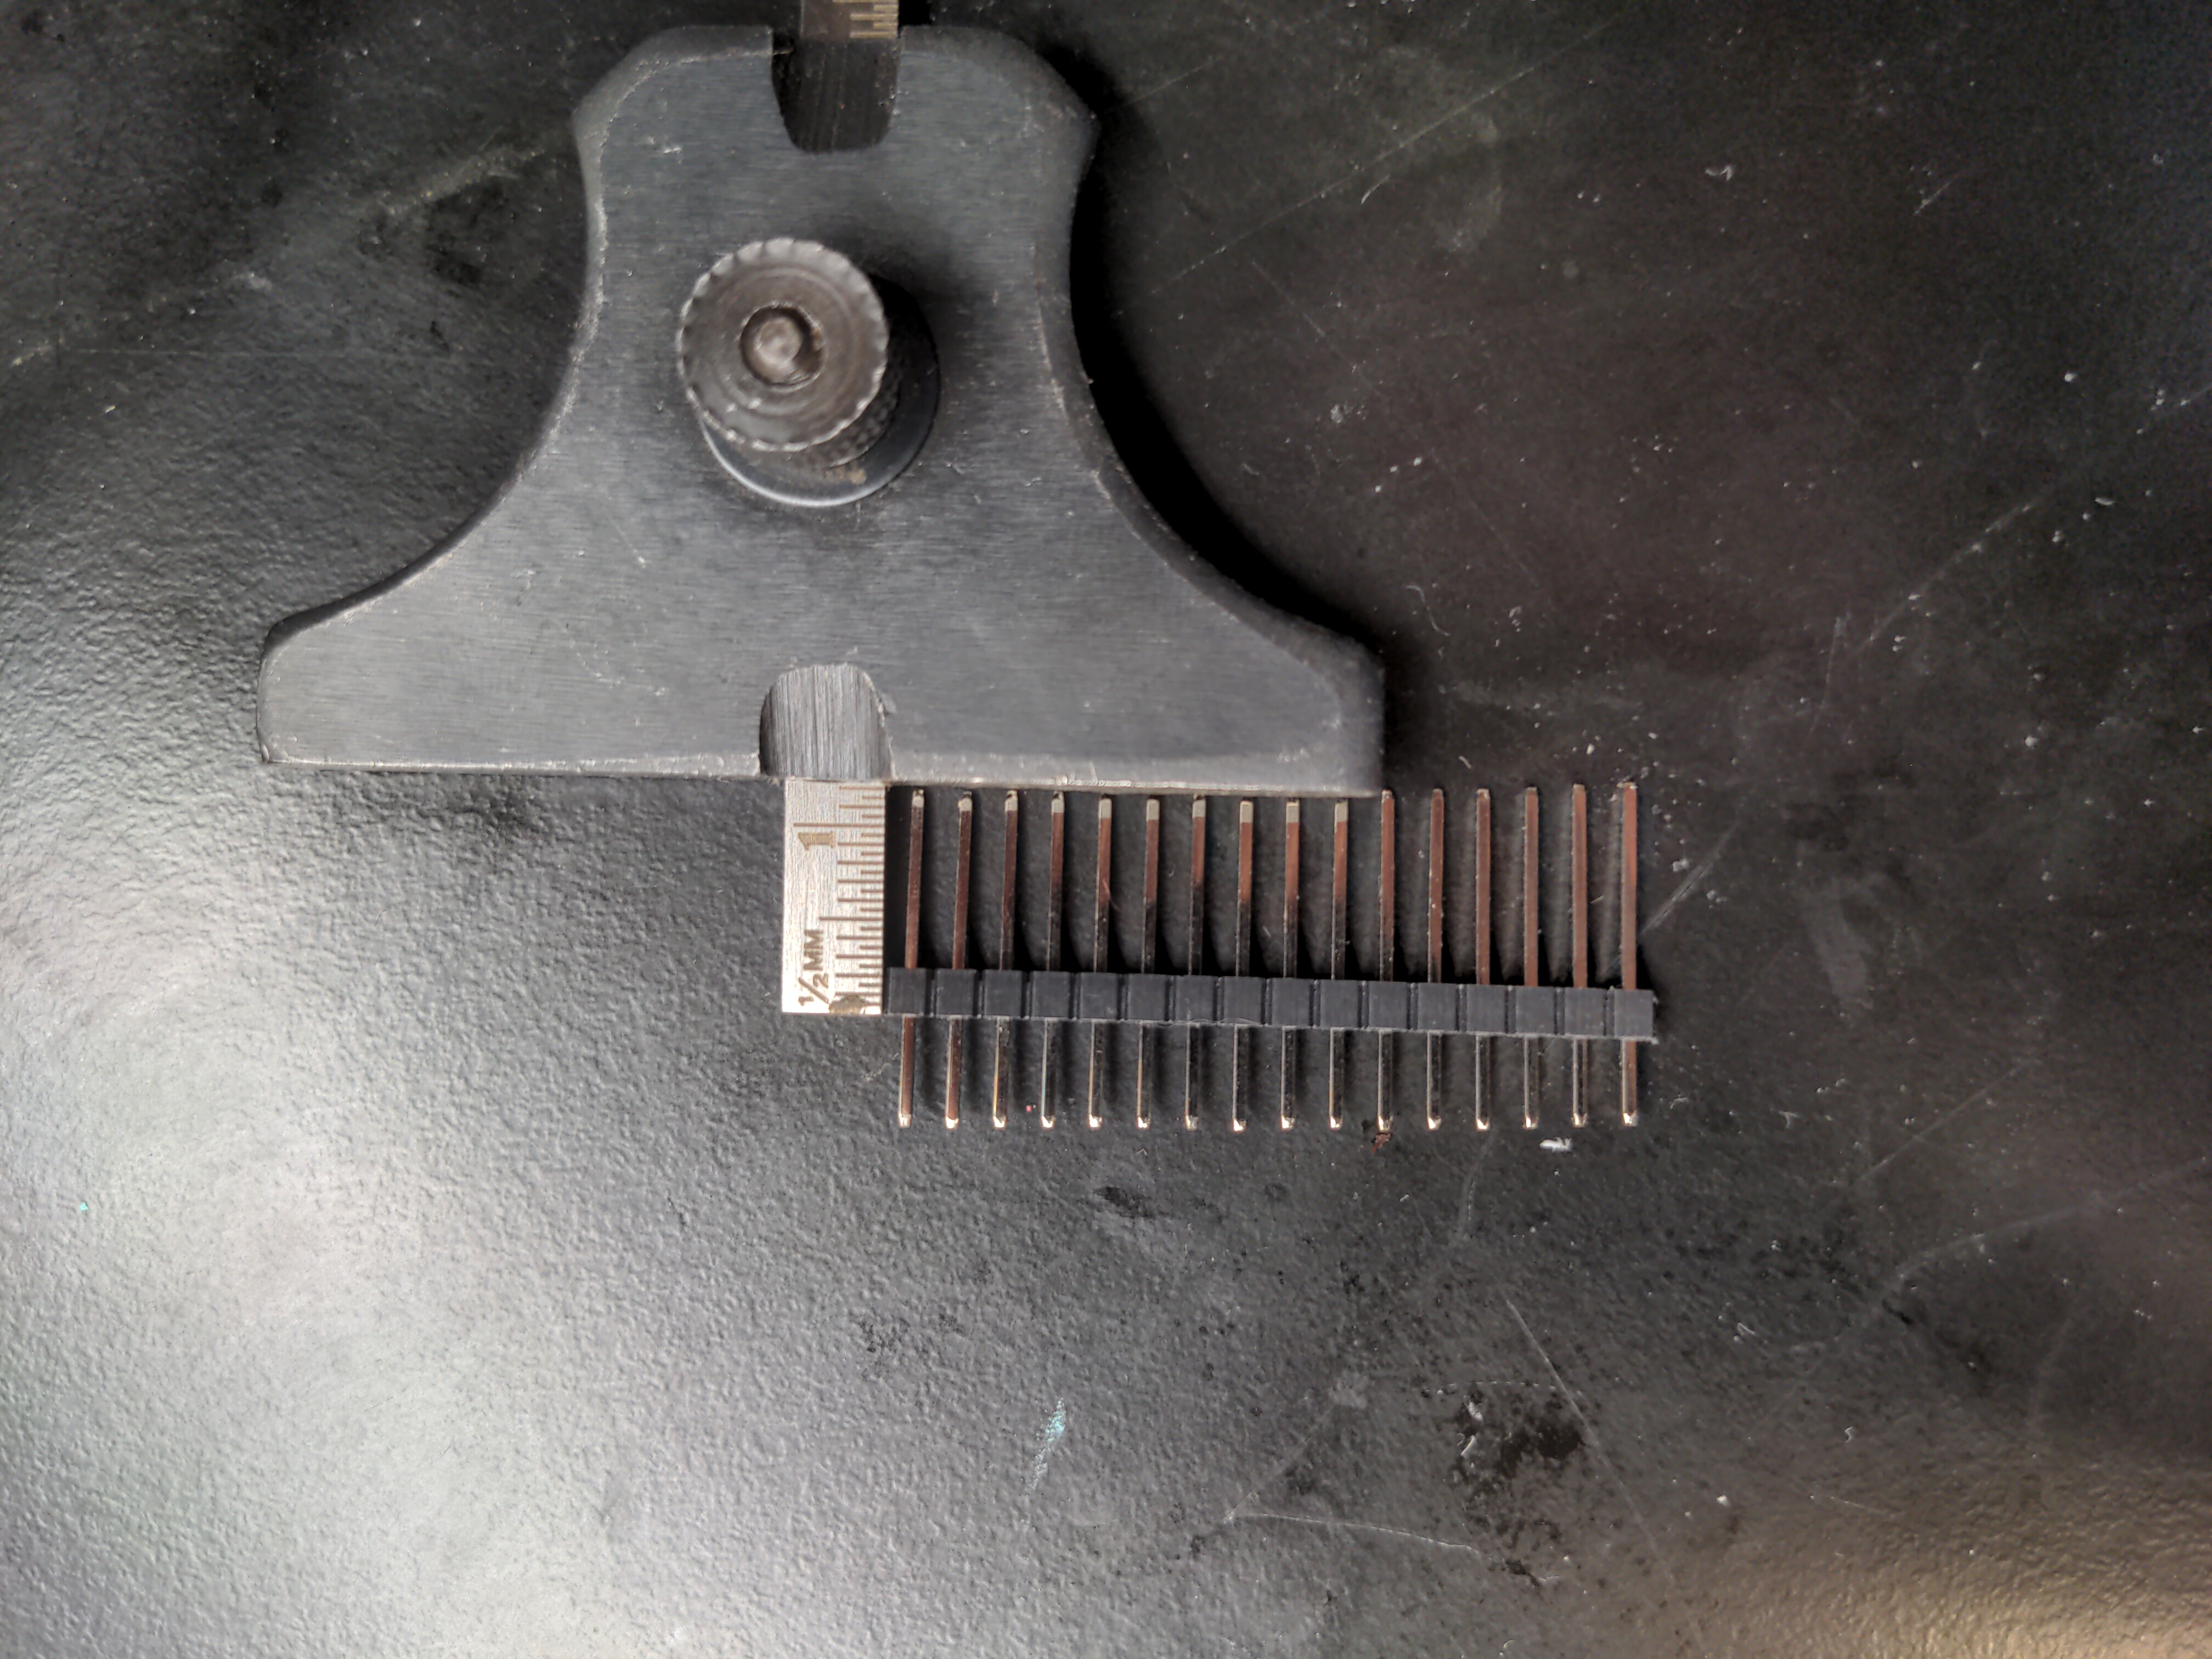
\includegraphics[width=3in]{img/modified_headers.jpg}
  \caption{All headers adjusted to be 12mm above the board}
  \label{fig:headers}
\end{figure}
\begin{figure}
  \centering
  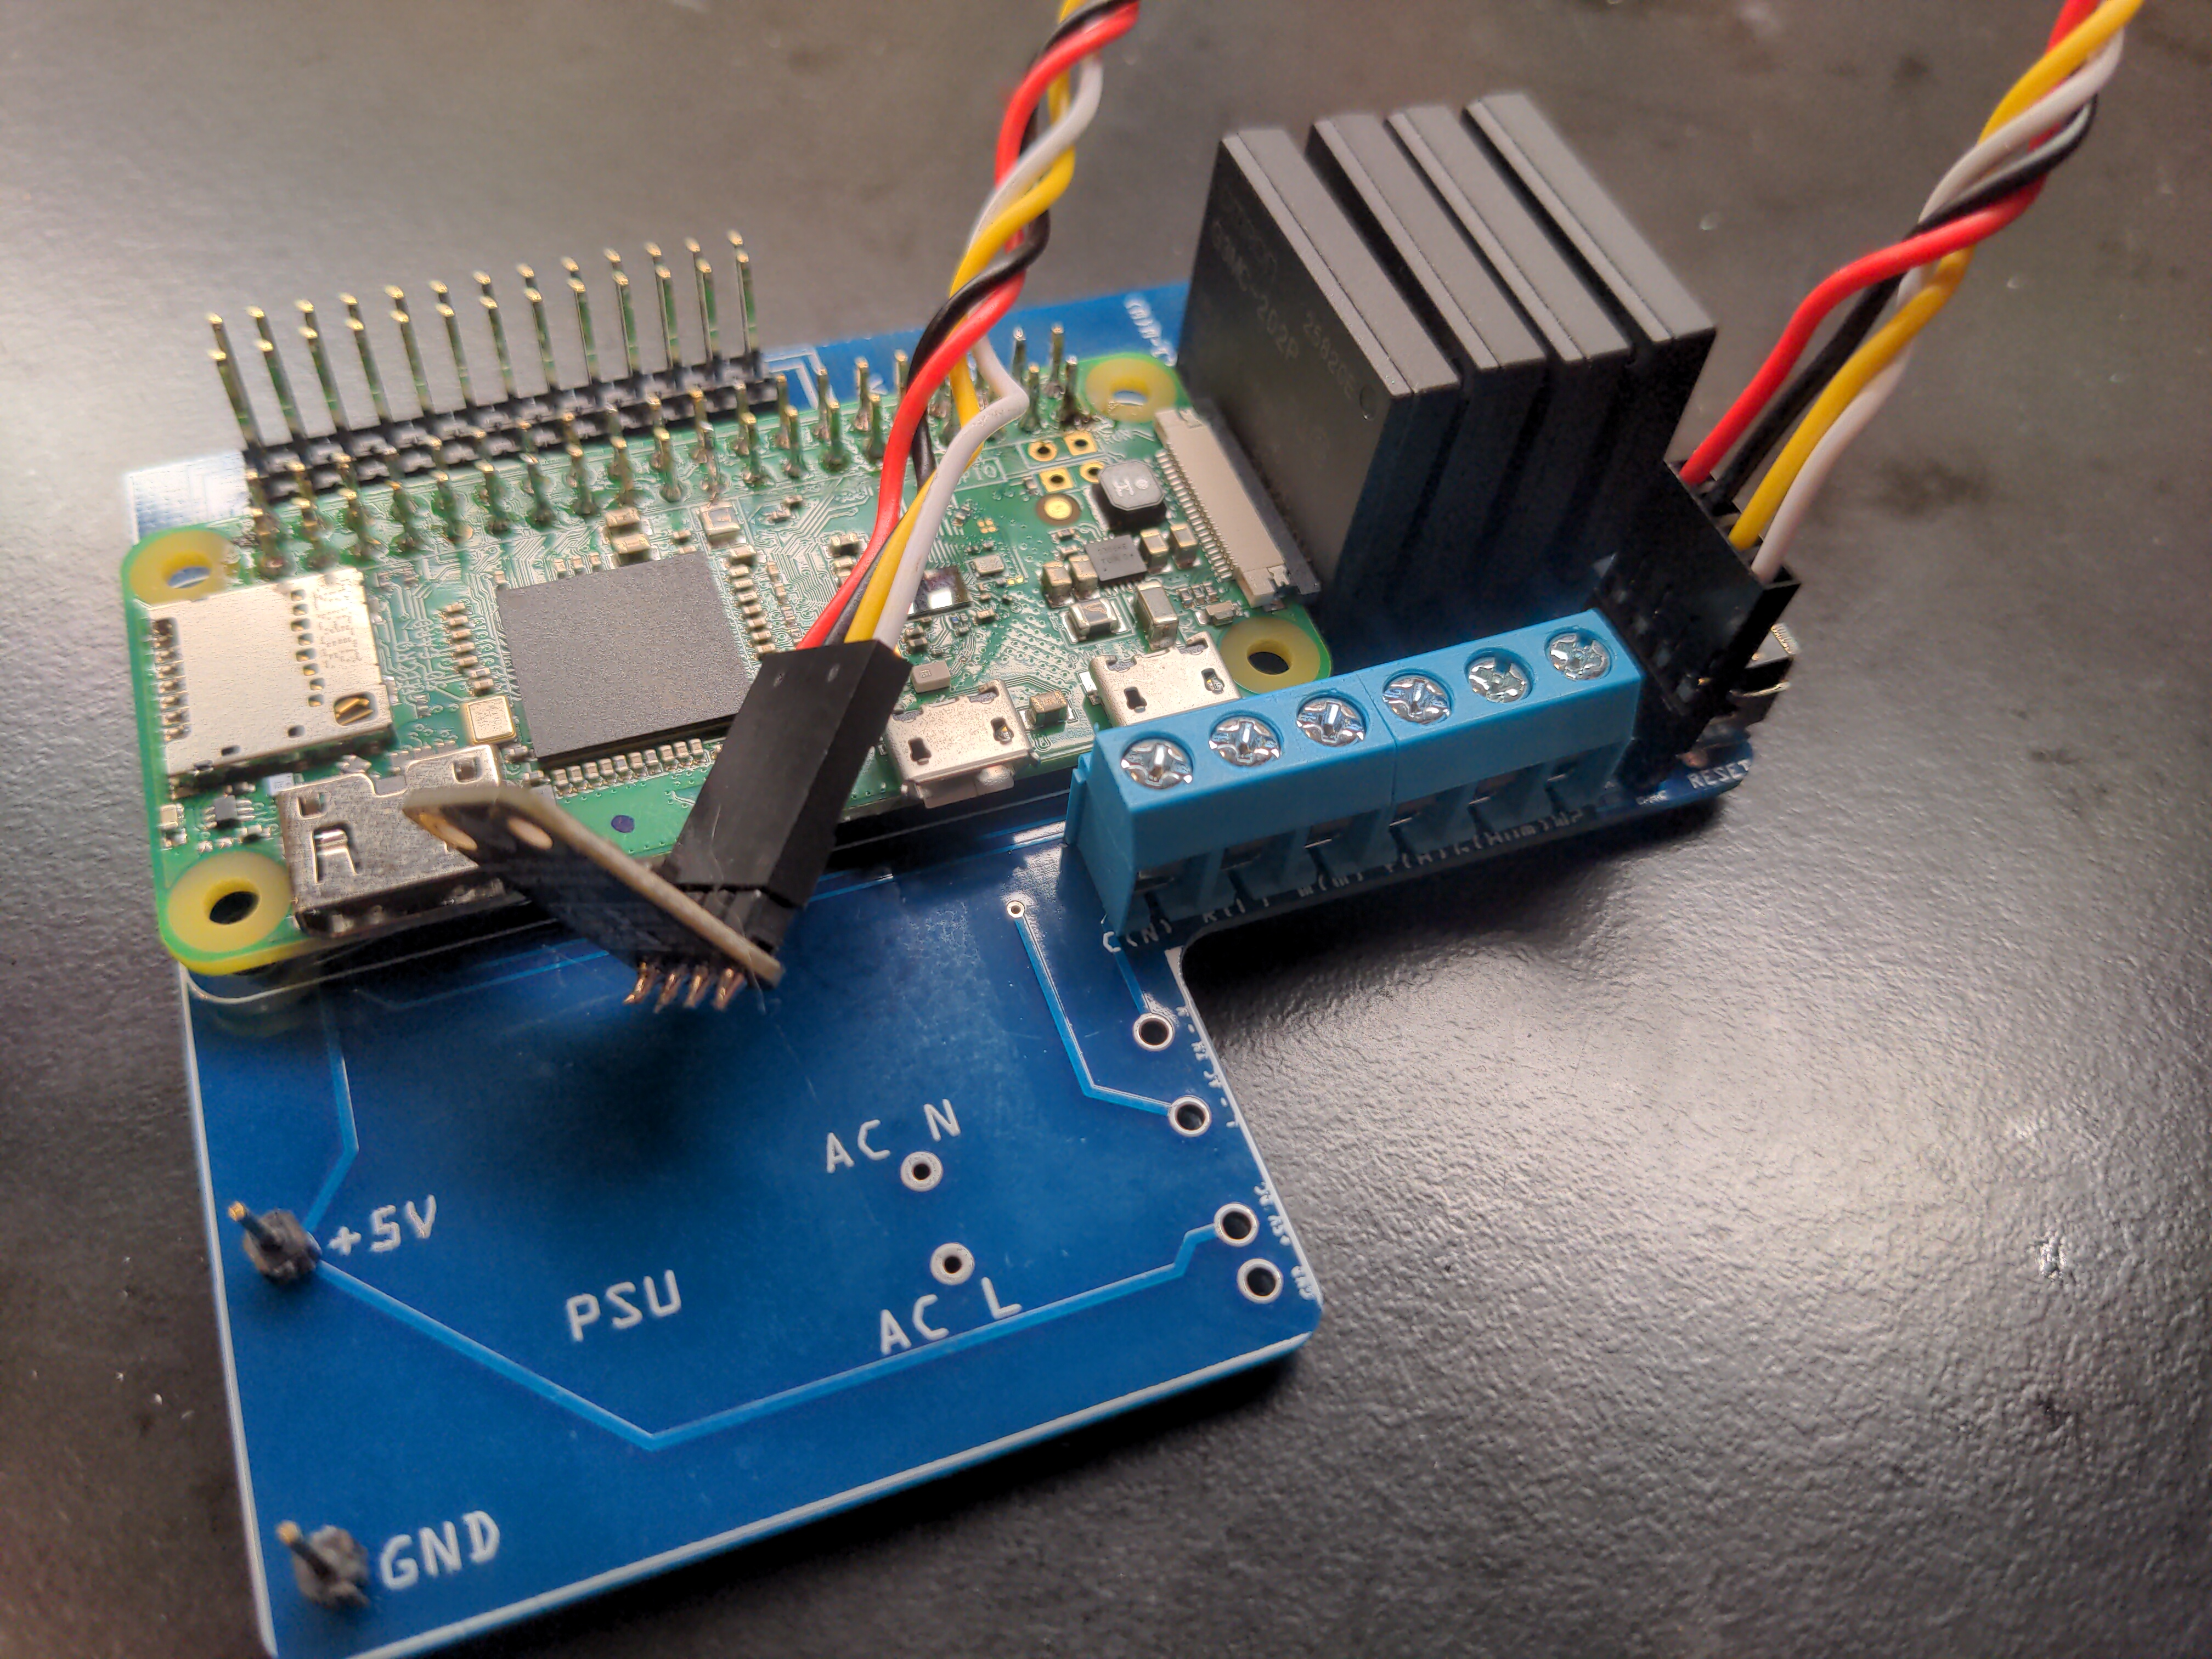
\includegraphics[width=3in]{img/fully_assembled.jpg}
  \caption{Fully assembled HestiaPi with headers for a DC power supply}
  \label{fig:fully_assembled}
\end{figure}

\subsubsection{Video}
\href{https://www.youtube.com/watch?v=gRcRINqT31g}{\includegraphics[width=5.0in]{img/hestiapi_one_soldering.jpg}}

\subsubsection{Hints and Tips}
The LCD needs to be connected before powering HestiaPi as it initialises on
boot only (otherwise it looks blank-white and touch events do not register) and
it may also cause a freeze or reboot due to power spike.

If you cannot control mains, that is having it off during all the time of
installation, our advise is to leave the SD card and LCD out, connect all
wires, partly (not fully) insert the SD and finish off case installation with
the LCD attached to the cover.

Once all is done, from outside of the case, push first the SD all the way in
(it does not lock-click in place) and then insert a non-metallic tool and press
the reset button from the right side. HestiaPi will boot and in about 10-15sec
the LCD will show some of the boot messages.

\subsubsection{Troubleshooting}
After assembling you HestiaPi, put in an SD card that has been flashed, attach
the touch screen and try booting it up.

If you get a blank screen, the pi might not be booting properly.  Make sure the
SD card was flashed properly.  A common mistake is to flash the image onto the
partition instead of the block device (e.g., /dev/sdb1 instead of /dev/sdb).

Test your reset button.  If it doesn't work, odds are it's either a faulty
component, or more likely a cold solder joint.  The former can be fixed by
replacing the part, and the latter by re-soldering the component onto the
board.  Use a multimeter to verify the switch works.  If it does, trace the
line to the pin on the pi to see if there is connectivity there.


\subsection{Printing the Case}
\input{printing_the_case}

\subsection{Wall Installation ONE} \label{Wall Installation ONE}
HestiaPi's case comes in 2 parts. The backplate that goes to the wall and
should not be visible and the front cover. The backplate should have 4 small
holes, 3 larger holes and an opening for the wires coming from the wall.

If you bought HestiaPi, all internal screws are replaced with plastic rivets.
Otherwise you would need:

\begin{itemize}
\item 4 x 2.5Mx25mm hex screws
\item 4 x 2.5M hex nuts
\end{itemize}

For attaching to the wall you need:
\begin{itemize}
\item 4 x 3.5Mx40mm non-countersunk screws
\end{itemize}

Place the hex screws through the 4 small holes entering from the side facing
the wall. Secure them in the hex slot and make sure they are sit flush. Remove
the LCD from the PCB and insert the PCB alone guiding the 4 screws through the
4 corner holes of the Pi and secure with the nuts. Avoid using a large tool.
You can simply tighten them by hand. Don't overtighten.

With the remaining 3 larger holes mark your wall and drill according to the
location of the wires. The opening of the backplate should match the location
of the wires. Secure the backplate and PCB with the 3 larger screws.

Complete wiring according to your model instructions (for US see Figure
\ref{fig:us}; for EU see Figure \ref{fig:eu})

\begin{figure}
  \includegraphics[width=5.0in]{img/US-hvac-wiring-diagram.jpg}
  \caption{US Wiring Diagram}
  \label{fig:us}
\end{figure}

\begin{figure}
  \includegraphics[width=5.0in]{img/eu-wiring-diagram.jpg}
  \caption{EU Wiring Diagram}
  \label{fig:eu}
\end{figure}

Remove any protective film from the LCD if present and lock the LCD on the
cover from the inside making sure the LCD's header is at the top.

Guide the 4 wires through the slit of bottom partition of the cover and secure
the sensor in it so that it is thermally protected from the rest of the
circuit.

If you installed the bottom screw it may block the cover to fully insert. Clip
off part of the sensor partition to allow enough clearance.

Hold the front cover aligned to the backplate and bring closer while you make
sure the pin header of the PCB is aligned to the header of the LCD. Push firmly
from the sides of the cover and not from the LCD till it locks in place. Make
sure no wires are caught in between as this may block the cover from locking in
place securely.



\section{Usage}
\subsection{Touchscreen} \label{Touchscreen}
\input{touchscreen}
\subsection{Webpage} \label{Webpage}
\input{webpage}
\subsection{Mobile app}
The interface for the mobile app is almost identical to the basic UI of the
webpage (covered in section \ref{Webpage}).  The only signficiant differences
are getting the application and connecting to the HestiaPi.

The application can be downloaded from
\href{https://f-droid.org/en/packages/org.openhab.habdroid/}{F-Droid}, the
\href{https://play.google.com/store/apps/details?id=org.openhab.habdroid&hl=en_US}
{Google Play store}, or \href{https://apps.apple.com/us/app/openhab/id492054521}
{Apple's App store}. Ideally, as long as your mobile device is connected to
the same network as the HestiaPi, the app should automatically find the
HestiaPi's OpenHAB server. If this works as expected, everything should look
similar to the screenshots shown in figure \ref{fig:Web UI}.

If the server is not found, the hamburger menu in the top left (three
horizontal lines) will bring up a menu that allows access to the settings.  In
the settings menu, there is a Local section which allows connecting to a local
OpenHAB server.  The app refuses to connect to unencrypted web servers when the
URL is entered manually, so the URL should be slightly different than described
in the web UI: \texttt{https://[YOUR\_HESTIA\_IP]:8443/}  Once the URL is
entered, return to the settings screen and in the local section, it should say
``Insecurely connected to \texttt{YOUR\_HESTIA\_IP}''.  It says the connection
is insecure because the app has no way to verify that the server is actually
the correct one.  The app will work fine when connected ``insecurely'' and to
get a secure connection requires quite a bit of effort and technical know-how.
For instructions on how to get the app to say it's a secure connection, see
the ``\nameref{Set up TLS}'' section (\ref{Set up TLS}).

Now that the application is connected to the server, click the back arrow to
return to the Main Menu.


\section{Configuration}
\subsection{First boot}
The first time you boot your HestiaPi, it will go through a setup process which
requires it reboot several times to set everything up.

Follow the on-screen instructions on the LCD when it prompts to connect your
phone to the ``HESTIAPI'' network with HESTIAPI as the password. Once connected
you will automatically be prompted on your phone (or computer) to select your
WiFi network from a list (no hidden SSID supported yet) and enter the password.
If you are not automatically taken you to the wifi setup screen, open
\url{http://192.168.4.1/} in a web browser. This should look similar to what is
in figure \ref{fig:wifi_setup}.

\begin{figure}
  \centering
  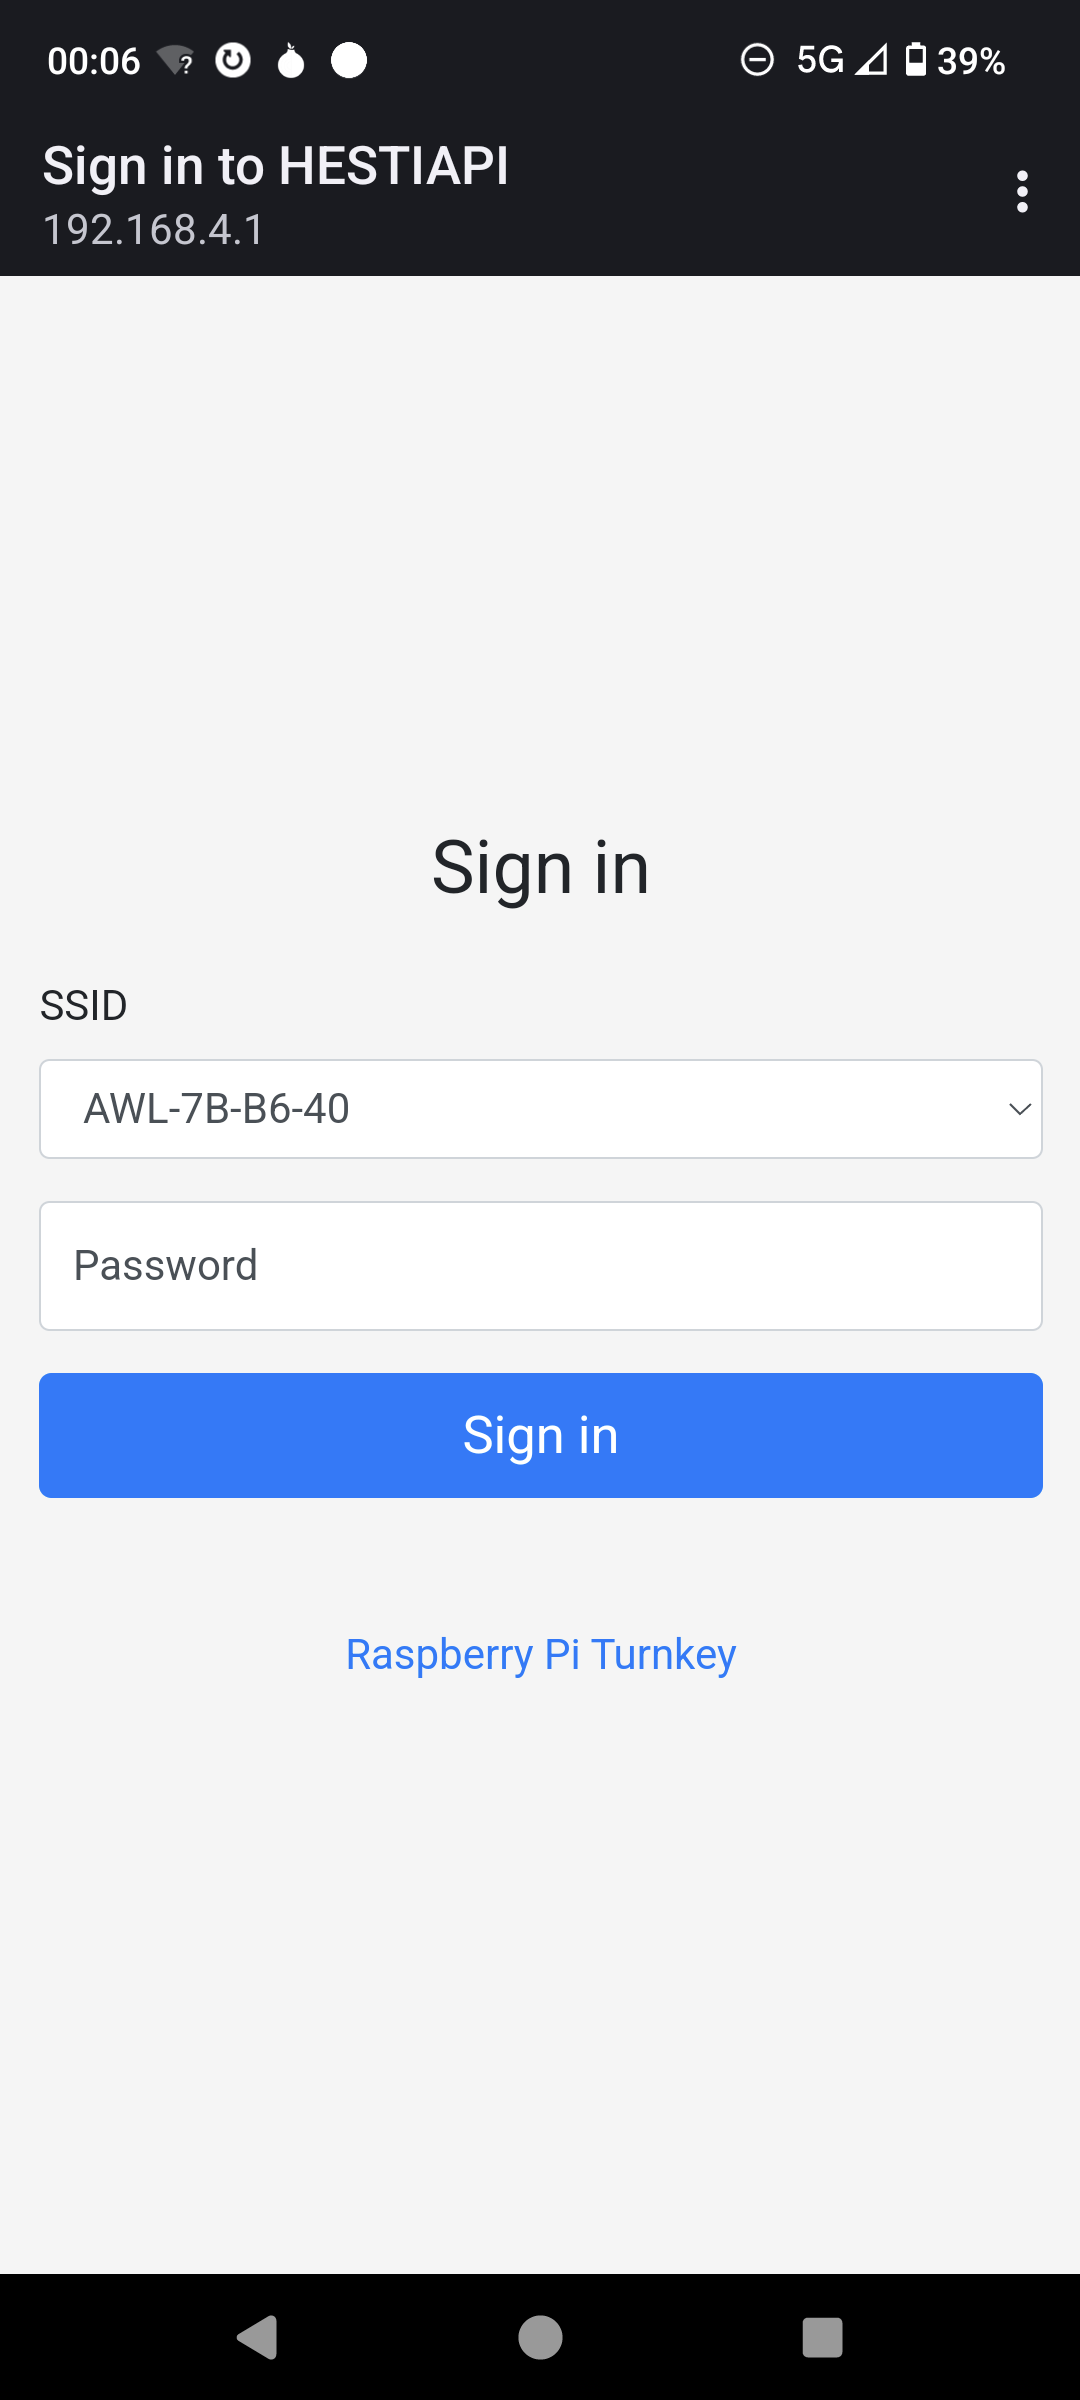
\includegraphics[height=3in]{img/wifi-setup.png}
  \caption{Screen for setting up the HestiaPi's wifi access}
  \label{fig:wifi_setup}
\end{figure}

If you entered the correct wifi info, your HestiaPi will restart and connect to
your network. You should no longer see the HESTIAPI network when you look for
wifi networks on your phone (or computer). The loading screen should show you
the IP address of the HestiaPi while it is booting, and that should be an IP
address from your home network (as opposed to being 192.168.4.1, which is what
it will be if the thermostat is not connected to your wifi network).

When selecting your access point, you will need to choose a 2.4GHz network.
Some routers use both 2.4GHz and 5GHz, however the Rasberry Pi inside of the
HestiaPi does not support 5GHz. This should not be a problem as routers are
configured to be compatible with both, however it's important to know if you
have changed your router settings to disable the 2.4GHz band.

From the time you first turn it on to the time that you are ready to use the
thermostat can take up to 20 minutes. While you are waiting, you may want to
download a mobile app to access the thermostat without having to navigate to
the HestiaPi using a web browser. See section \ref{Mobile App} for more
details.

When the HestiaPi first boots, the LCD UI may start with zeros for the
temperature and humidity. This is normal and the data will update in a minute
or two. If your HestiaPi is using a temperature sensor that does not also have
the ability to sense humidity, the humidity reading will remain as 0\%.

Once the LCD is showing the UI with temperature values, try and load the mobile
app or use your phone or laptop and navigate to:
http://[hestiapi\_IP]:8080/start/index (substituting in your HestiaPi's IP
address where appropriate) and select ``Basic UI''.

You should now be able to control the basic functions from either the app or
your browser.

OpenHAB2 has a great \href{https://community.openhab.org/}{forum} with loads of
information from fellow users who are willing to help you customize your system
to suit your needs.

Please note that the UI of the app, web and LCD may change with software updates
so be sure to back up any customizations you make before running an update.

\subsection{Boot Sequence}
On startup, the HestiaPi will run a number of services, which does take some
time due to the low computational power of the pi.  However, booting is
something which very infrequently done, which is why the boot times of five
minutes or more are acceptable in order to keep the size and cost of the
hardware low.

%Understanding the startup process requires understanding what components are
%running.  The components are documented in section \ref{Software Architecture}.

Systemd starts up a number of services, including:
\begin{enumerate}
  \item mosquitto
  \item hciuart
  \item dhcpcd
  \item openhab2
\end{enumerate}

The status of sll of these services can be checked with
"\texttt{systemctl status SERVICENAME}" where SERVICENAME is replaced with the
name of the service of interest. For example, to check the status of Mosquitto:
\texttt{systemctl status mosquitto}

In addition to things started by systemd, there are also scripts which are run
from /etc/rc.local.


\subsection{Connect WiFi}
Follow the on-screen instructions on the LCD when it prompts to connect your
phone to the ``HESTIAPI'' network with HESTIAPI as the password. Once connected
you will automatically be prompted on your phone to select your WiFi network
from a list (no hidden SSID supported yet) and enter the password. This should
look similar to what is in figure \ref{fig:wifi_setup}).

Your HestiaPi will then restart to connect to your network and the HESTIAPI
network will not be shown again if you entered the correct the details.

\begin{figure}
  \centering
  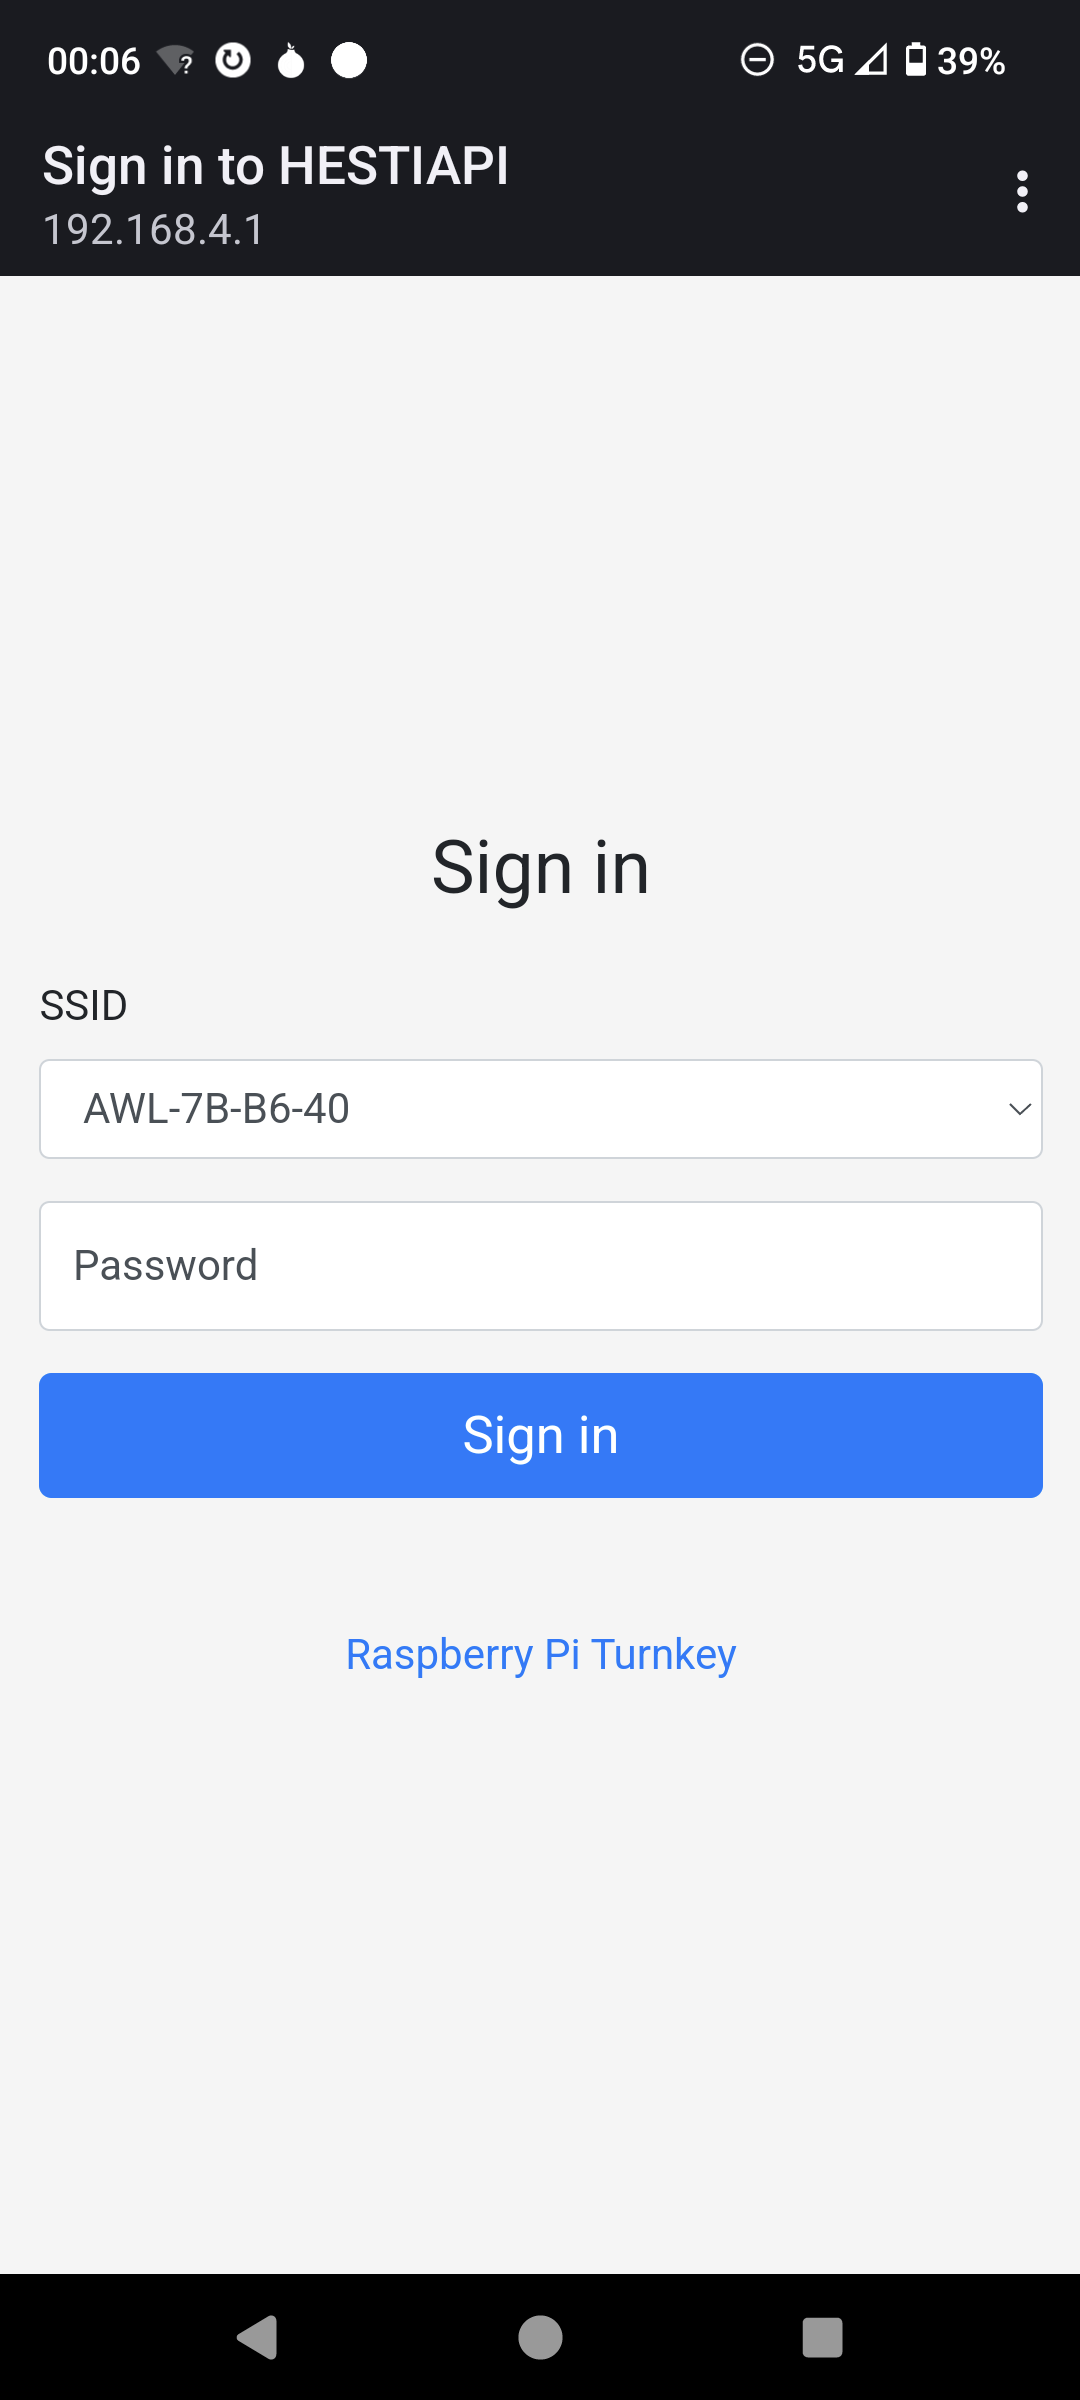
\includegraphics[height=3in]{img/wifi-setup.png}
  \caption{Screen for setting up the HestiaPi's wifi access}
  \label{fig:wifi_setup}
\end{figure}

\subsection{Change Settings}
\subsubsection{Easy Remote Access}
All latest releases of HestiaPi offer very easy remote access to your home
without touching your network modem/router or even knowing HestiaPi's IP! Does
not depend on port forwarding or DynDNS! Woohooo!

\textbf{Please note that this is an externally hosted service not controlled by
you or us but by OpenHAB itself.}

\href{https://www.youtube.com/watch?v=joz5f4ejJVc}{Instructions video} (if you
prefer video to text)

To activate it (shipped disabled by default for obvious reasons) go to
http://[YOUR-HESTIAPI-IP]:8080/paperui/index.html and select Add-ons > MISC and make
sure ``openHAB Cloud Connector'' is installed.

Once installed SSH into your HestiaPi (username: pi and password: hestia) and
type:

\texttt{    cat /var/lib/openhab2/uuid}

 copy the output somewhere. Then type:

\texttt{        cat /var/lib/openhab2/openhabcloud/secret}

copy this output too. Reboot your HestiaPi

\texttt{        sudo reboot}

    
Then go to \url{https://myopenhab.org} and create an account using your details
and the above information (UUID and secret).

You can now access your HestiaPi Touch from a browser or your mobile app

Hint: Enter \url{https://myopenhab.org} as a remote url and your myopenHAB
account username and password as credentials

\subsubsection{Update Your DynDNS Automatically}
By default, the HestiaPi does not connect to any external servers. If you want
the thermostat to tell a dynamic DNS service about the its publis IP address,
the
\href{https://github.com/HestiaPi/hestia-touch-openhab/blob/ONE/home/pi/scripts/getpublicip.sh}
{getpublicip.sh} script can help you do just that.

The file is already on your HestiaPi at:

\texttt{/home/pi/scripts/getpublicip.sh.bak}

You will need an account with whatever service you choose to use inside the
script, and the will need to be modified to specify your username, password
and possibly domain name. There are some example in the script near the bottom
which are commented out. Customize and uncomment them and then rename the
script to \texttt{getpubliship.sh} and you should be good to go. This file is
already run periodically by OpenHAB.

Note: Old versions of the HestiaPi software automatically reached out to
ipinfo.io to determine your public IP address. For these versions, the script
is already named \texttt{getpublicip.sh} and so you just have to edit that
file to get it to report the public IP to your dynamic DNS provider.

\subsection{Setting a Static IP Address} \label{Static IP}
\input{static_ip}
\subsection{Set up TLS} \label{Set up TLS}
Setting up Transport Layer Security (TLS) is an advanced topic which requires
owning a domain, having control over a DNS server, the ability to forward ports
on the edge router, setting up web servers, and using the command line.  As
such, it is recommended that only people who are at least somewhat familiar
with these technologies attempt to set this up.  For the vast majority of
users, setting up TLS is not necessary, and it is safe to skip this step.

At the core, setting up TLS just means giving the server a host/domain name,
getting a trusted certificate for that name, and accessing the server by name
instead of by IP address.  The rest of this section assumes the reader is
familiar with how to SSH into their HestiaPi and switch user to be root.

The example provided here is just one way to get a TLS certificate, and the
method described prioritizes making sure the HestiaPi is never directly
accessible from the Internet.  This ensures that random people in the internet
will not be able to modify your home automation system.

Figure \ref{fig:tls-overview} shows the overall setup.  In this example, we
will use the domain example.org.  You will need to replace this domain with one
that you control.  The process involves setting up a web server which will
publicly be known as hestia1.example.org.  This web server will be directly
connected to the internet and is what will obtain the TLS certificate.  The
public DNS server will resolve hestia1.example.org to your public IP address.
This is needed because the certificate authority (LetsEncrypt in our example)
will reach out to the hostname to verify that it really is who it claims to be.
Once the web server has the TLS certificate, it can be copied over to the
HestiaPi to be used there.  The final component is an internal DNS server,
which is used for devices on the LAN to connect to the HestiaPi by name and it
needs to be given the internal IP address.  It is possible to configure some
DNS servers to give out different results depending on who it asking (e.g. the
public IP if the router asks, but the LAN IP if the request comes from anywhere
else on the LAN), but this documentation chose to have two separate servers in
an attempt to make the configurations less complex.

\begin{figure}
  \includegraphics[width=\textwidth]{img/tls_overview.png}
  \caption{Complicated TLS Setup Overview}
  \label{fig:tls-overview}
\end{figure}

\subsubsection{Static IP}
To assign the HestiaPi a static IP address, see section \ref{Static IP}.

\subsubsection{DNS Servers} \label{DNS Servers}
Setting up a DNS server is beyond the scope of this document.  There are many
guides which have been written on the topic, such as
\href{https://www.debuntu.org/how-to-setting-up-a-dns-zone-with-bind9/}{this}.
If you have a bind9 server, adding an entry for the HestiaPi in the internal
DNS server might look like this:

\begin{verbatim}
hestia1                 IN      A       10.1.1.31
\end{verbatim}

The external entry would look the same, but it would be your public IP address
instead of the HestiaPi's internal IP address.  The internal DNS server will
also need to be configured to do recursive DNS lookups.  This is typically
set in \texttt{/etc/bind/named.conf.options} using something like the
following instide the \texttt{options} section:

\begin{verbatim}
allow-recursion { 10.1.1.0/24; localnets; };
allow-query { 10.1.1.0/24; localnets; };
allow-query-cache { 10.1.1.0/24; localnets; };
recursion yes;
\end{verbatim}

For more details on how this works, read
\href{https://www.zytrax.com/books/dns/ch7/queries.html}
{documentation about bind9} or
\href{https://serverfault.com/questions/634546/bind9-proper-recursion-setup/634564#634564}
{this stackoverflow post}.

Updating your computers and mobile devices to point to this name server is best
done at the router.  Instructions for making this change will vary from one
router to the next, but your router's documentation should explain how to change
the nameservers that the DHCP server is assigning.

Once the entry has been added to the nameserver and your computer or device is
using that nameserver, you should be able to access the HestiaPi by name.  In
the example above, the host name would be hestia1 and the domain used in the
linked blog post is debuntu.foo.  This means opening a browser and going to:
\texttt{http://hestia1.debuntu.foo:8080/}

\subsubsection{Obtain TLS certificate}
In order to avoid connecting the HestiaPi to the internet where anyone could
interact with it, this guide shows how to obtain a trusted TLS certificate
using a web server.  At this point it's expected that a public DNS server has
been configured to point to your public IP address (see section
\ref{DNS Servers}).

The next step is to set up a Linux server which will act as the web server.
Once Linux is intalled, you'll need to set up a web server, such as
\href{https://www.nginx.com/resources/wiki/start/topics/tutorials/install/}
{nginx}.  Consult your router's documentation on how to forward port 80 from
your router to the web server.  At this point you should be able to access the
webpage from the internet.  An easy way to test this is to use a mobile phone
or tablet with cell data service.  Disconnect from wifi and attempt to go to
hestia1.example.org and verify there's a web server running.  This verifies
that the DNS, port forwarding and web server are all working correctly.

Follow the \href{https://certbot.eff.org/instructions}{instructions} on how to
use certbot to obtain a TLS certificate.  The
\href{https://letsencrypt.org/docs/}{LetsEncrypt Documentation} is rather
comprehensive and can provide additional context to how their system works.

Once complete, there should be a directory in \texttt{/etc/letsencrypt/live}
for your hostname which contains links to the TLS certificates.

\subsubsection{Configure HestiaPi to use new Certificate}
In order to use your new certificate, it needs to be converted from PEM format
to pkcs12 format and imported to the Java keystore, after deleting the previous
certificate.  At this point you should have two files: one with the private key
for your certification, and the other should be your public certificate and any
intermediate certificates that browsers will need to verify your certificate.
With letsencrypt, these files are named privkey.pem and fullchain.pem.

First, we convert these to pkcs12 format and put them into a single file, with
the password that the HestiaPi is going to expect (``openhab'').

\begin{verbatim}
openssl pkcs12 -export -inkey privkey.pem -in fullchain.pem -out openhab.p12 -passout pass:openhab
\end{verbatim}

Next, we want to stop openhab so we aren't modifying a file that is in use, and
we delete the key that is there (whose alias is mykey), and add the .p12 file
that we just created.

\begin{verbatim}
# Lets not modify a keystore that is in use...
sudo systemctl stop openhab2
# Delete the old key
sudo /opt/jdk/zulu8.40.0.178-ca-jdk1.8.0_222-linux_aarch32hf/bin/keytool \
        -keystore /var/lib/openhab2/etc/keystore \
        -v -storepass openhab -delete -alias mykey
# Import the new key
sudo /opt/jdk/zulu8.40.0.178-ca-jdk1.8.0_222-linux_aarch32hf/bin/keytool \
        -keystore /var/lib/openhab2/etc/keystore -importkeystore \
        -srckeystore ~/openhab.p12 -srcstoretype PKCS12 \
        -destkeystore /var/lib/openhab2/etc/keystore -deststoretype jks \
        -destalias mykey -srcalias 1 -srcstorepass openhab -deststorepass openhab
\end{verbatim}

In the event you want to look to see what is in the keystore, you can do so
with the following command:

\begin{verbatim}
# List keys (for debugging)
/opt/jdk/zulu8.40.0.178-ca-jdk1.8.0_222-linux_aarch32hf/bin/keytool \
       -keystore /var/lib/openhab2/etc/keystore \
       -v -storepass openhab -list
\end{verbatim}

Finally, we start openhab2 and it may take a while for the web server to start,
but when it does, it should be using the new certificate.

\begin{verbatim}
sudo systemctl start openhab2
\end{verbatim}

Navigate to your hostname (e.g., \texttt{http://hestia1.debuntu.foo:8443/}) and
you should have an encryped connection to your HestiPi!



\subsection{File Structure \& Paths}
\subsubsection{GPIO pin mappings}

\textbf{Relays}

\begin{tabular}{|c|c|c|}
\rowcolor{lightgray}
\hline
         & \textbf{Pin} & \textbf{GPIO} \\ 
\hline
 Relay 1 & 32           & GPIO12 \\ 
\hline
 Relay 2 & 16           & GPIO23 \\  
\hline
 Relay 3 & 12           & GPIO18 \\
\hline
 Relay 4 & 36           & GPIO16 \\
\hline
\end{tabular}

\textbf{Temperature sensor}

The BME or BMP sensor can be at either I2C address 0x76 or 0x77. The software
will check both addresses, in this order.

\begin{tabular}{|c|c|c|}
\rowcolor{lightgray}
\hline
     & \textbf{Pin} & \textbf{GPIO} \\ 
\hline
 SDA & 3            & GPIO02 \\ 
\hline
 SCL & 5            & GPIO03 \\ 
\hline
\end{tabular}

\textbf{LCD touchscreen pinout}

\begin{tabular}{|c|c|c|}
\rowcolor{lightgray}
\hline
\textbf{Pin no.} & \textbf{Symbol} & \textbf{Description} \\ 
\hline
1, 17 & 3.3V & Power positive (3.3V power input) \\ 
\hline
2, 4 & 5V & Power positive (5V power input) \\ 
\hline
3, 5, 7, 8, 10, 12, 13, 15, 16 & NC & Not connected \\ 
\hline
6, 9, 14, 20, 25 & GND & Ground \\ 
\hline
11 & TP\_IRQ & Touch Panel interrupt, low level while the Touch Panel detects touching \\ 
\hline
18 & LCD\_RS & Instruction/Data Register selection \\
\hline
19 & LCD\_SI/TP\_SI & SPI data input of LCD/Touch Panel \\
\hline
21 & TP\_SO & SPI data output of Touch Panel \\
\hline
22 & RST & Reset \\
\hline
23 & LCD\_SCK/TP\_SCK & SPI clock of LCD/Touch Panel \\
\hline
24 & LCD\_CS & LCD chip selection, low active \\
\hline
26 & TP\_CS & Touch Panel chip selection, low active \\
\hline
\end{tabular}


\subsubsection{Configuration files}

\textbf{WiFi details}

\texttt{/etc/wpa\_supplicant/wpa\_supplicant.conf}

\textbf{OpenHAB}
Items

\texttt{/etc/openhab2/items/default.items}

Rules

\texttt{/etc/openhab2/rules/default.rules}

Sitemaps

\texttt{/etc/openhab2/sitemaps/default.sitemap}

Things

\texttt{/etc/openhab2/things/default.things}

Logs

\texttt{/var/log/openhab2/events.log\\
/var/log/openhab2/openhab.log}

\textbf{LCD UI}
The LCD UI is an HTML-based page loaded on a fullscreen browser. All HTML, CSS, JS, fonts and icon files are in here

\texttt{/home/pi/scripts/oneui}

The vue framework is used.
    
\textbf{Scripts}
In 
\texttt{/home/pi/scripts}

There are
\texttt{AdafruitDHTHum.py\\
AdafruitDHTTemp.py}

Read sensor data from DHT sensors.

\texttt{C2F.sh\\
F2C.sh}

Change HestiaPi from Celcius to Fahrenheit and vice versa.

\texttt{getBMEhumi.sh\\
getBMEtemp.sh\\
getBMEpress.sh}

Read sensor data from BME sensors (calling bme280.py).

\texttt{getcputemperature.sh}

Returns RasPi CPU temperature.

\texttt{getssid.sh}

Returns WiFi SSID name.

\texttt{gettz.sh}

Returns system Timezone.

\texttt{getuseddiskspace.sh}

Returns used SD card space.

\texttt{getwifiinfo.sh }

Returns WiFi signal strength.

\texttt{getwlan0ip.sh }

Returns WiFi IP.

\texttt{getwlan0mac.sh }

Returns WiFi MAC address.

\texttt{netcheck.sh }

Cron script that checks WiFi connectivity by pinging its gateway. If no
response is received at the first time, the WiFi interface is restarted and a
DHCP (dynamic) IP is requested. If no response is received again RaspberryPi,
the reboot command is sent. Please note this script is not enabled by default
and you will need to follow the instructions supplied at the top of the file.
Please also note that restarting the Pi will stop any current task and will not
resume after restart.

\texttt{openhabloader.sh }

Loads the Touch LCD UI.

\texttt{getpublicip.sh }

Checks current public IP and if it matches with previous reading, it does
nothing else. If current public IP is different, the latest value is sent to
your account (manual and free account registration needed).
    
\textbf{Web UI}

\texttt{http://[YOUR\_HESTIA\_IP]:8080/basicui/app}

or simply


\texttt{http://[YOUR\_HESTIA\_IP]:8080}

and then select Basic UI and default

\textbf{Smartphone App}
Under Settings > Local server settings


\texttt{http://[YOUR\_HESTIA\_IP]:8080}



\section{FAQ}
\subsection{Configuration}
\subsubsection{Default SSH Username and Password}

Username: pi

Password: hestia

SSH port: 22

\subsubsection{MQTT Configuration}
All the topics are defined in the .things
\href{https://github.com/HestiaPi/hestia-touch-openhab/wiki/File-Structure-&-Paths-ONE}{file}.

Confirm by subscribing from another laptop to all (\#) MQTT IDs and listen for
published messages while you play with your HestiaPi. For Linux users, run this
in a terminal:

\texttt{mosquitto\_sub -h [HESTIA\_PI\_IP] -d -t hestia/\#}

\subsubsection{How to Access My HestiaPi From Outside My House}

You will need a WiFi router with port forwarding feature (most routers do these
days) and if you don’t have a static IP (or if you don’t know what this is),
you will need to use a free Dynamic DNS service called
\href{https://www.noip.com/support/knowledgebase/install-ip-duc-onto-raspberry-pi/}{NoIP}.
Don’t worry -- although we can’t offer support on individual routers, we can
certainly point you in the right direction. Installation instructions on the
above link.  Alternatively you can use my.openhab.org which is a service hosted
externally and is not controlled by us or you but by OpenHAB itself. Go to:

\texttt{http://[YOUR-HESTIAPI-IP]:8080/paperui/index.html}

and select Add-ons > MISC and install ``openHAB Cloud Connector'' if not
installed. Once installed SSH into your HestiaPi (username: pi and password:
hestia) and type:

\texttt{cat /var/lib/openhab2/uuid}

write the output down. Then type:

\texttt{cat /var/lib/openhab2/openhabcloud/secret}

write this output down too.

Then go to \url{https://myopenhab.org} and create an account using your details
and the above information (UUID and secret). You can now access your HestiaPi
Touch from a browser or your mobile app (enter ``\url{https://myopenhab.org}''
as a remote url and your myopenHAB account username and password as
credentials).  The above steps are also available in youtube format
\href{https://www.youtube.com/watch?v=joz5f4ejJVc}{here} too.


\subsection{Troubleshooting}
\subsection{General issues}
For those who are having problems and don't want to read the entire
troubleshooting section, just try reflashing the SD card with the latest image
from \url{https://hestiapi.com/downloads}. This really will fix nearly every
problem! So if your issue isn't listed, or you just want a quick fix, re-flash
that SD card and you'll likely be back in business in no time.

\subsection{Verifying relay status}
If you are unsure if the relays are turning on or off when they should, this
can be checked in software. To do so, you will need to be able to SSH into the
HestiaPi.

To determine if a relay on, SSH into the pi and then look at the GPIO value.
The mappings of which GPIO pins are connected to which relays are in section
\ref{GPIO pin mappings}.

As an example, relay 1 is GPIO12, which is the fan for HVAC systems and
humidity when in Generic (EU) mode. After SSHing into the HestiaPi, the command
below would display a ``1'' if that function was on, or a ``0'' if it was off.

\texttt{cat /sys/class/gpio/gpio12/value}

If this reports that the relay is on, but the the fan (or humidity for EU
systems) is not on, it indicates that there's likely an issue with wiring or
with your HVAC system.

If this reports that the functionality is off, when you think it should be on,
you may want to manually turn it on. After SSHing into the HestiaPi, you will
need to become root, and then set the GPIO value. To continue with the fan
example on HVAC systems, here are commands you would run after SSHing into the
pi in order to turn the fan on, and then turn it back off again.

\texttt{sudo su -\\
echo 1 | /sys/class/gpio/gpio12/value \# turn on\\
echo 0 | /sys/class/gpio/gpio12/value \# turn off\\
}

As soon as you run the ``echo 1'' command, the fan should turn on. There should
not be any delay. The same should be true when running the command to turn off
the relay.

Turning on relays in this manner bypasses the thermostat logic, which means
that the function will never turn off. That's why it's important to make sure
to manually turn off the functionality after you manually turn it on. If you
forgot to turn off the cooling system after manually turning it on, it'd likely
burn out the compressor, which would be a very expensive repair.

Running these commands should help you in determining if there is an issue with
the hardware or with the software. If these command do not cause the functions
to turn on, it points to a hardware issue, such as incorrect wiring.

If these commands work as expected but the heat does not turn on when the
heating set point is higher than the temperature, and the heating system is
turned on, it indicates that something is going wrong in the software (more
specifically, in OpenHAB). If that's the case, you can get help on the forum
at \url{https://community.hestiapi.com/}. Please be patient, as we are all
volunteers and it may be a few days before we see your message and have time to
investigate and reply.

\subsection{Eternal loading screen}
If your thermostat ever reboots and the loading countdown on the screen goes
all the way down to the point where it just says ``Loading...'' and stays there
for hours, it's either a software issue or a slow micro SD card.

First, reflash the SD card and this will almost certainly have you back up and
running.

If that does not work, the only other potential cause we have seen is using an
old, generic, or slow SD card. Using a card rated at 10MB/sec should be
sufficient, and 30MB/sec would be ideal. Unlabeled cards, or ones rated at
lower speeds may work. We have not found a card that will consistently cause
this issue, so we can't say for sure what the minimum acceptable speed is.

An icon that looks like a 10 inside a circle, a 1 inside a letter U, or a V10
are all icons that mean it's 10MB/sec. A 3 inside a U, or V30 indicated it is
a 30MB/sec card. There are faster cards, labeled V60 and V90, but getting a
card that fast is not necessary.

\subsection{Taps do not register on the touchscreen}
If the screen doesn't turn on, see the entry below about that. These steps are
to troubleshoot situations where the display is working correctly, but just not
responding to touches.

This most often is caused by a pinched screen. This can be either the tabs of
the case pinching the screen too tightly or the case pinching down on the front
of the screen. First, look for any wires that may have gotten pinched between
the relays or power supply (the tall components) and the screen when the case
was snapped into place. This is the most common cause of this issue and
fortunately it is easily resolved.

To confirm that it is a pinch, connect the screen without the shell of the case
and power on the HestiaPi. If it works correctly, this tells us that the case
is to blame.

To determine if it's the shell pinching down when it is closed, remove the
HestiaPi from the case's backplate, then connect the screen while it is in the
case's shell. Do not snap on the backplate. If the touchscreen works in this
configuration, we know the tabs that hold the LCD to the shell are not the
problem.

If the screen does not work with the backplate off, we know that the tabs are
pinching the screen too tightly. In this case, the tabs can be very carefully
scraped down with a hobby knife, box cutter, file or something of this nature.
Take care not to break of the tabs or hurt yourself.

If you are in a situation where the shell of the case is pinching down on the
screen only when it's connected with the backplate (and there are no wires
getting in between the screen and the rest of the HestiaPi), it means the case
is a bad fit. One option is to not quite snap the case completely shut. The LCD
pins will hold the shell in place and it should work fine. The next option is
to run without the shell on, which will give you a very punk look to your
thermostat. Or you can get a custom printed shell for your case that is slightly
taller.

If you are an advanced user and want to try to try to resolve this issue, the
tails of the headers on the back of the main PCB can sometimes be trimmed to
get just a tiny bit more room, which is often all that is needed. The PCB
should generally be as close to the backplate as possible. Another possibility
is to trim all of the LCD headers to make them just a little bit shorter. This
will make it even more difficult to align the pins when putting the case on,
but people have successfully repaired their thermostats by doing this.

Other causes of the touchscreen not registering taps include: the Raspberry Pi
was powered on when the LCD screen was connected improperly, someone pushed on
the screen too hard, or only some of the pins are fully connected to the
screen. If the touch part of the screen is broken, the above tests will all
have the same results (no response to taps). At this point, your options are to
replace the screen or just use the screen for viewing information and make all
the changes to the thermostat over wifi.

\subsection{Screen doesn't turn on}
If you see lights illuminated on the pi, but the screen doesn't turn on at all,
the screen is not receiving power, which means it is likely not connected
properly. Look in through the side of the case and see if you can tell if the
pins are aligned correctly. If you can not determine this, try removing the
shell of the case and connect the screen on without the shell of the case. The
screen should light up slightly when powered on. If this still doesn't work, it
is likely a defective screen. If you have another Raspberry Pi available, you
can connect it to the top left pins of the Pi (when the SD card is on the left)
and see if the screen lights up when that Pi is powered on with the HestiaPi's
SD card in it.

If the screen lights up slightly, but is blank, this is a different issue. In
this case, the screen is likely working and it's an issue with the software.
You should see the screen flicker within 60 seconds and you should see the
boot messages after a few minutes.

The fastest and easiest fix is to just copy the image onto the SD card again
and try again. If you are an advanced user and want to spend time
troubleshooting the issue to determine the root cause, we encourage you to
share whatever you find with the community at
\url{https://community.hestiapi.com}.

\subsection{Screen is slow to respond to taps}
The HestiaPi should respond to touches within a second. If it's responding
to taps, but it taking a long time, it's likely a software issue. In this
case, copying a fresh image onto the SD card will likely fix it. The other
thing that can be done to get it to respond faster to touches is to get the
fastest SD card available.

A video has been made to demonstrate how quickly the screen should respond to
taps. A stylus is used here to make it clear when the tap is occurring versus
when the screen is updating, but it should work the same when tapping with your
finger. \url{https://peertube.gsugambit.com/w/1AhKQByTrAg38HKSQUJFR3}

\subsection{How to edit files via SSH}
If you are very new to command line interface we would advise you taking a
short online course by searching for ``linux command line interface'' on your
favourite website.

To edit a file while you are inside SSH use the command

\texttt{sudo nano /path/to/your/file}

Then leave your mouse alone as it does not control you cursor anymore

Use only your keyboard and once you are done, press Ctrl+O to save and Ctrl+X to close.

\subsection{Start OpenHAB2 in Debug Mode}

For OpenHAB2 (v10.x image -- July 2018)
To monitor the OpenHAB logs without stopping the service run

\texttt{openhab-cli showlogs}

To start OpenHAB manually after stopping the service run

\texttt{openhab-cli start}

For older OpenHAB installations:
Stop OpenHAB first

\texttt{sudo service openhab2 stop}

and when it is stopped, start it manually

\texttt{/usr/share/openhab2/start\_debug.sh}

once (if) loaded type inside the OpenHAB session

\texttt{log:tail}

and notice any issues.


\end{document}

